%  Licensed to the Apache Software Foundation (ASF) under one
%  or more contributor license agreements.  See the NOTICE file
%  distributed with this work for additional information
%  regarding copyright ownership.  The ASF licenses this file
%  to you under the Apache License, Version 2.0 (the
%  "License"); you may not use this file except in compliance
%  with the License.  You may obtain a copy of the License at
%  
%  http://www.apache.org/licenses/LICENSE-2.0
%  
%  Unless required by applicable law or agreed to in writing,
%  software distributed under the License is distributed on an
%  "AS IS" BASIS, WITHOUT WARRANTIES OR CONDITIONS OF ANY
%  KIND, either express or implied.  See the License for the
%  specific language governing permissions and limitations
%  under the License.

\documentclass{article}
\setcounter{tocdepth}{2}

\usepackage[utf8]{inputenc}
\usepackage[ngerman]{babel}

\usepackage[pdftex]{graphicx}
\usepackage{listings}
\usepackage[svgnames]{xcolor}
\usepackage{hyperref}

\definecolor{mygreen}{RGB}{1,121,111} %pinegreen
\pagestyle{plain}

% listings for uima ruta
%%%%%%%%%%%%%%%%%%%%%%%%%%%%%%%%%%%%%%%%%%%%%%%%

\definecolor{rutaAction}{rgb}{0,0,0.5}%0,0,128 bold
\definecolor{rutaBasic}{rgb}{0.5,0.5,0.5}%128,128,128 bold
\definecolor{rutaCondition}{rgb}{0,0.5,0}%0,128,0 bold
\definecolor{rutaDeclaration}{rgb}{0.5,0,0}%128,0,0 bold
\definecolor{rutaString}{rgb}{0.16,0,1}%42,0,255
\definecolor{rutaComment}{rgb}{0.24,0.5,0.37}%63,127,95

\renewcommand{\lstlistingname}{UIMA Ruta Quelltext}

\lstnewenvironment{Ruta}[1][]
    {\lstset{float=htpb,#1}} 
    {}
\lstset{
	language=Java,
    basicstyle=\normalfont\ttfamily\scriptsize,
	%caption=Descriptive Caption Text,
	%label=DescriptiveLabel
 	frame=L,
    %rulesepcolor=\color{blue},
	% xleftmargin=.5in,
    % xrightmargin=.5in,
    %rulesep=.2in,
    framesep=.1in,
    captionpos=t,
    numbers=none,                   % where to put the line-numbers
    numberstyle=\tiny\color{gray},  % the style that is used for the line-numbers
    showstringspaces=false,
    %rutaAction
    keywords=[2]{DEL, CALL, MARK, MARKSCORE, COLOR, LOG, REPLACE,      FILLOBJECT, RETAINTYPE, SETFEATURE, ASSIGN, PUTINLIST, ATTRIBUTE, MARKFAST,      FILTERTYPE, CREATE, FILL, MARKTABLE, UNMARK, TRANSFER, MARKONCE, TRIE,      GATHER, EXEC, MARKLAST, ADD, REMOVE, MERGE, GET, GETLIST, REMOVEDUPLICATE, GETFEATURE, MATCHEDTEXT, CLEAR, UNMARKALL, SHIFT, CONFIGURE, DYNAMICANCHORING, TRIM, ADDRETAINTYPE, REMOVERETAINTYPE, ADDFILTERTYPE, REMOVEFILTERTYPE, MARKFIRST},
    keywordstyle=[2]\color{rutaAction}\bfseries,
    %rutaBasic
    keywords=[3]{ALL, ANY, AMP, BREAK, W, NUM, PM, Document,
      MARKUP, SW, CW, CAP, PERIOD, NBSP, SENTENCEEND, COLON, COMMA, SEMICOLON, WS, SPACE, SPECIAL, EXCLAMATION, QUESTION},
    keywordstyle=[3]\color{rutaBasic}\bfseries,
    %rutaCondition
    keywords=[4]{CONTAINS, IF, INLIST, PARTOF, TOTALCOUNT, CURRENTCOUNT, CONTEXTCOUNT, LAST, VOTE, COUNT, NEAR, REGEXP, POSITION, SCORE, ISLISTEMPTY, MOFN, AND, OR, FEATURE, PARSE, IS, BEFORE, AFTER,      STARTSWITH, ENDSWITH, PARTOFNEQ, SIZE, NOT},
    keywordstyle=[4]\color{rutaCondition}\bfseries,
    %rutaDeclaration
    keywords=[5]{WORDLIST, DECLARE, BOOLEAN, PACKAGE, TYPE, TYPESYSTEM, INT, DOUBLE, FLOAT, STRING, SCRIPT, WORDTABLE, ENGINE, BLOCK, RULES, BOOLEANLIST, INTLIST, DOUBLELIST, FLOATLIST, STRINGLIST, TYPELIST, UIMAFIT, IMPORT, FROM},
    keywordstyle=[5]\color{rutaDeclaration}\bfseries,
    commentstyle=\color{rutaComment},       % comment style
    stringstyle=\color{rutaString}   % string literal style
 }

%%%%%%%%%%%%%%%%%%%%%%%%%%%%%%%%%%%%%%%%%%%%%%%%


\title{Detecting mentions of characters in German novels with Apache UIMA{\texttrademark} Ruta\\
(in German)
}

\begin{document}

\maketitle


\tableofcontents

\section{Einleitung}

In diesem Tutorial wird die regelbasierte Skriptsprache UIMA Ruta anhand eines Beispiels vorgestellt. Das Ziel ist es, jedes Vorkommen einer Person (Vorname, Nachname etc.) in einem literarischen Text zu annotieren. Zunächst werden die Programme Eclipse, UIMA Ruta und TreeTagger installiert und konfiguriert. Zur Einführung in die Entwicklung werden grundlegende Elemente der Sprache Ruta erläutert und die Ordnerstruktur innerhalb eines Projekts beschrieben. Anschließend wird das erste Kapitel eines Romans auf eindeutige Muster untersucht, um wichtige Merkmale zum Auffinden von Personen zu erhalten. Die Erläuterung verschiedener Regeln soll dabei helfen, die Syntax zu verstehen und Grundtechniken kennenzulernen. Nachdem TreeTagger vollständig in ein Projekt integriert wurde, können mehr Typen zur Regelentwicklung genutzt werden. Zum Schluss wird der \textit{Annotation Test} in die Entwicklung miteinbezogen, der das Testen der Regeln automatisiert. Speziell hierfür wird ein vorher markiertes Referenzdokument benötigt.

\section{Installation}

\subsection{Eclipse}
Wir rufen zunächst die Internetpräsenz \url{www.eclipse.org} auf. Dort klicken wir auf den Reiter \textit{Downloads} oder die Schaltfläche \textit{Download Eclipse}. Auf der nachfolgenden Seite wird das Paket \textit{Eclipse Standard} heruntergeladen. Zuvor müssen wir noch das entsprechende Betriebssystem und den Systemtyp auswählen. In Windows finden wir die Information unter \textbf{Windows $\rightarrow$ Computer $\rightarrow$ Rechts\-klick $\rightarrow$ Eigenschaften} im Abschnitt \textit{System}. Wenn wir das Paket heruntergeladen haben, muss es, z.B. mit dem freien Packprogramm 7-Zip\footnote{\url{http://www.7-zip.org/}}, entpackt werden. In dem entpackten Ordner ist die Datei \textit{eclipse.exe}, mit der die Anwendung gestartet wird. Beim Start von Eclipse muss ein Ordner angegeben werden, in den alle Projekte gespeichert werden. Mit Klicken auf \textit{Use this as the default and do not ask again} werden wir nicht bei jedem Start aufgefordert einen Arbeitsplatz anzugeben.

\subsection{UIMA Ruta}
Wir befinden uns nun auf der Arbeitsoberfläche von Eclipse und wollen UIMA Ruta installieren. Dazu navigieren wir zu \textbf{Help $\rightarrow$ Install New Software...}. Anschließend erstellen wir unter \textit{Add...} ein neues Repository mit dem Link \url{http://www.apache.org/dist/uima/eclipse-update-site/}. Jetzt wird nach den Paketen von UIMA Ruta gesucht und vor dem Eintrag \textit{Apache UIMA Ruta} ein Haken gesetzt. Wir bestätigen zweimal und akzeptieren die Lizenzbedingungen. Daraufhin wird das Programm mit allen benötigten Paketen installiert. Nachdem Eclipse neu gestartet wurde, kann die UIMA Ruta Workbench benutzt werden. Im Fenster rechts oben klicken wir noch auf das Fenstersymbol mit dem Plus und bestätigen den Eintrag UIMA Ruta, um die Perspektive zu wechseln.

\subsection{TreeTagger}\label{tt}
TreeTagger weist jedem Wort einer Wortart zu und bestimmt dessen Grundform. Die Wortarten sind dann in UIMA Ruta als Typen verfügbar und können in den Regeln benutzt werden. Wir laden uns das Programm auf der Internetseite \url{http://www.cis.uni-muenchen.de/~schmid/tools/TreeTagger/} unter der Überschrift \textit{Windows version} herunter. Außerdem werden für die Entwicklung deutscher Texte die deutschen Parameterdateien benötigt. Nachdem wir alles entpackt haben, kopieren wir die Parameterdateien in den Unterordner \textit{lib}. Jetzt erstellen wir eine Kopie von der größeren \textit{german-utf8.par} Datei und benennen sie in \textit{tagger-de-litte-endian.par} um. Danach wird ein neues Textdokument mit dem Inhalt \glqq encoding=utf8\grqq{} erstellt. Diese erhält den selben Namen, hat jedoch die Dateiendung \glqq .properties\grqq{}. Dabei ist darauf zu achten, dass der Dateityp in den Eigenschaften anschließend \textit{PROPERTIES-Datei} und nicht \textit{Textdokument} ist. Damit UIMA Ruta den Part-of-speech Tagger auf dem Datenträger findet, muss ein neuer Eintrag in den Umgebungsvariablen von Windows erstellt werden. Wir klicken auf \textbf{Windows $\rightarrow$ Computer $\rightarrow$ Rechtsklick $\rightarrow$ Eigenschaften} und links im Reiter auf \textbf{Erweiterte Systemeinstellungen}. Dort kann unter \textit{Umgebungsvariablen...} eine neue Systemvariable erstellt werden. Diese muss den Namen \glqq TREETAGGER\textunderscore HOME\grqq{} haben und als Wert den Speicherort von TreeTagger, also beispielsweise \glqq C:\textbackslash Programme\textbackslash TreeTagger\grqq{}.

\section{Erste Schritte}

\subsection{Die UIMA Ruta Workbench}
Nach der Installation von Eclipse und UIMA Ruta befinden wir uns auf der Arbeitsoberfläche von Eclipse (Abb.~\ref{workbench1}). Die Arbeitsoberfläche ist zunächst aufgeteilt in vier Bereiche. Auf der linken Seite ist der \textit{Script Explorer}, in dem sämtliche Projekte verwaltet und in einer hierarchischen Struktur angezeigt werden. Unten und auf der rechten Seite gibt es verschiedene Teilbereiche, die beispielsweise Fehler in der Programmsyntax anzeigen. Die wichtigsten Teilbereiche für unser Beispiel sind der \textit{Selection View}, der \textit{Annotation Test} und der \textit{Annotation Browser View}. Der obere Teil der Arbeitsoberfläche ist der eigentliche Arbeitsbereich. Hier werden die Regeln für das NER-System entwickelt, aber auch die markierten Dokumente angezeigt oder bearbeitet.

\begin{figure}
\centering
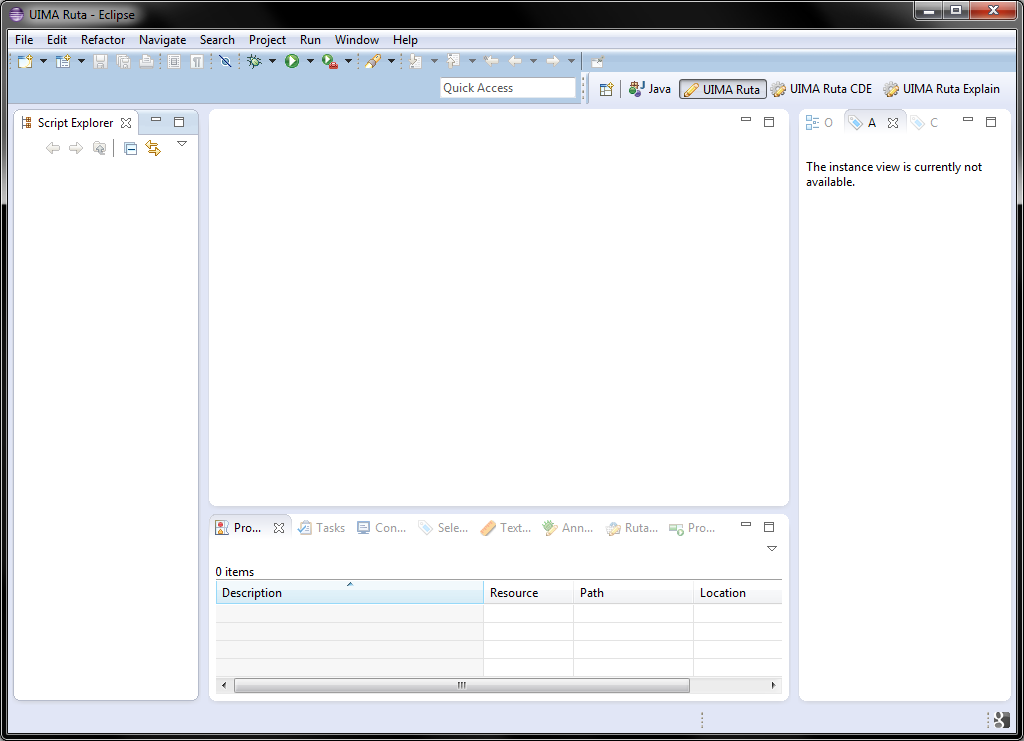
\includegraphics[width=0.5\textwidth]{figs/capture(1).png}
\caption{Die UIMA Ruta Workbench.}
\label{workbench1}
\end{figure}

Bevor wir loslegen, sollte noch die  Textkodierung in den Einstellungen von Eclipse geändert werden. Dazu rufen wir die Einstellungen mit \textbf{Window $\rightarrow$ Preferences} auf (Abb.~\ref{pref}). Anschließend navigieren wir zu \textbf{General $\rightarrow$ Work\-space} und ändern bei \textit{Text file encoding} den Eintrag in \textit{UTF-8}.

\begin{figure}
\centering
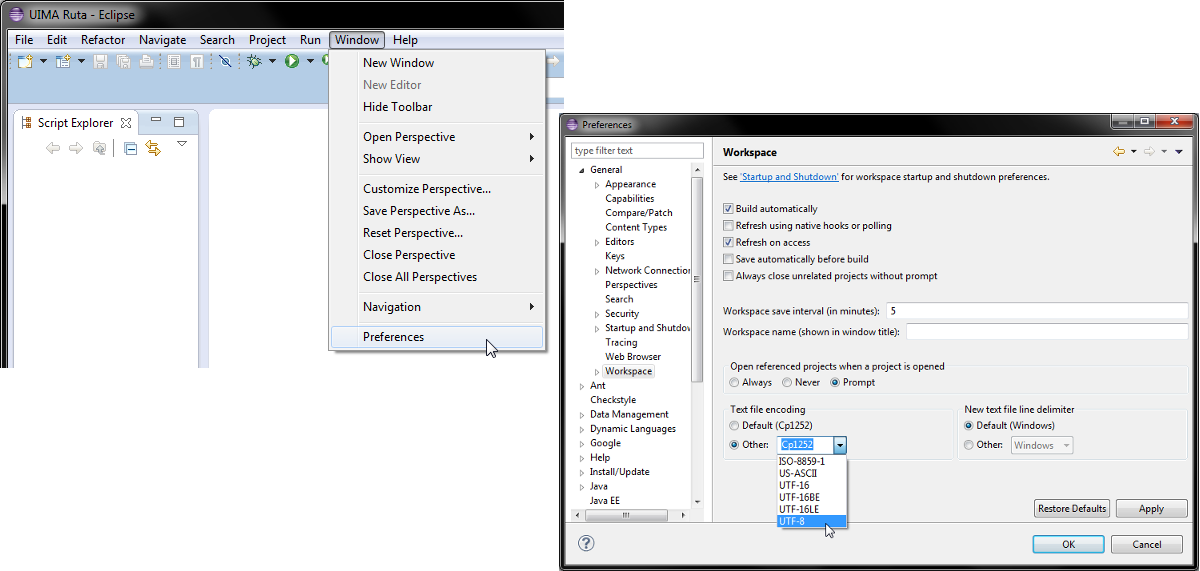
\includegraphics[width=1\textwidth]{figs/capture(2+3).png}
\caption{Die Einstellungen von Eclipse aufrufen und die Textkodierung ändern.}
\label{pref}
\end{figure}

\subsection{Das erste Projekt}\label{first_project}
UIMA Ruta organisiert die Projekte im \textit{Script Explorer} auf der linken Seite der Arbeitsoberfläche. Um ein neues Projekt zu erzeugen klickt man in einen freien Bereich des \textit{Script Explorers} mit \textbf{Rechtsklick $\rightarrow$ New $\rightarrow$ UIMA Ruta Project} (Abb.~\ref{newproject}). Im folgenden Fenster muss jetzt nur noch ein passender Name für das Projekt eingegeben und mit \textit{Finish} bestätigt werden. UIMA Ruta erstellt daraufhin das Projekt mit allen nötigen Ordnern. Das ausgeklappte Projekt mit der vordefinierten Ordnerstruktur wird in Abb.~\ref{folders} gezeigt. Das Projekt untergliedert sich in die Ordner \textit{script}, \textit{descriptor}, \textit{input}, \textit{output}, \textit{resources} und \textit{test}.

\begin{figure}
\centering
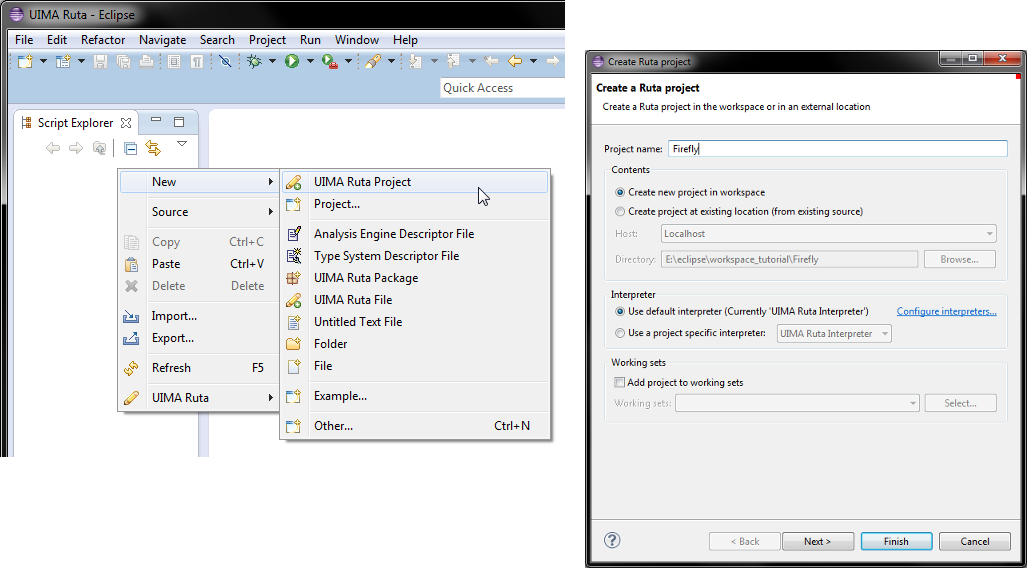
\includegraphics[width=1\textwidth]{figs/capture(4+5).png}
\caption{Ein neues Projekt erstellen und einen Namen angeben.}
\label{newproject}
\end{figure}

Im \textit{script} Ordner werden alle UIMA Ruta Skripte und Pakete gespeichert, die im Laufe der Programmentwicklung entstehen. Das Analysewerkzeug und die verschiedenen Typesystems von UIMA Ruta befinden sich in \textit{descriptor}. Hier können auch eigene Typesystems eingefügt und benutzt werden. Als Anfänger sollte allerdings nichts verändert werden, da sonst unerwartete Fehler auftreten könnten. In \textit{input} speichert man die Texte, die von den Skripten bearbeitet werden sollen. Dies können Text-, HTML- oder XMI-Dateien sein. XMI-Dateien sind von UIMA Ruta erstellte Textdokumente, die bereits mit Annotationen versehen sind. Die vom Skript annotierten Dateien werden dann im \textit{output} Ordner als XMI-Dateien gespeichert. Auf jede Datei im \textit{input} Ordner folgt eine Datei in \textit{output}. UIMA Ruta bietet die Möglichkeit Wortlisten, Wörterbücher oder Tabellen zur Regelentwicklung einzubeziehen. Diese Zusatzdateien werden im Ordner \textit{resources} gespeichert, damit UIMA Ruta darauf zugreifen kann. Zum Evaluieren der Regeln gibt es den Ordner \textit{test}. Hier werden markierte XMI-Dokumente in den jeweiligen Ordnern als Referenz gespeichert. Der \textit{Annotation Test} prüft dann, wie gut die aktuellen Regeln auf die Texte zugeschnitten sind.

\begin{figure}
\centering
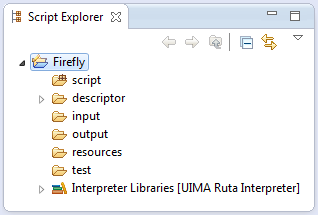
\includegraphics[width=0.5\textwidth]{figs/capture(6).png}
\caption{Das neue Projekt mit vordefinierter Ordnerstruktur.}
\label{folders}
\end{figure}

Ist ein größeres Projekt geplant, kann der Ordner \textit{script} noch weiter in sog. Pakete aufgeteilt werden. Um ein neues Paket zu erstellen, klickt man einfach auf \textit{script} mit \textbf{Rechtsklick $\rightarrow$ New $\rightarrow$ UIMA Ruta Package} (Abb.~\ref{newpack}). Der Name wird dann im nächsten Fenster mit \textit{Finish} bestätigt.

Die Ansicht der Paketstruktur kann störend sein, wenn bei jedem Start von Eclipse durch die Pakete geklickt werden muss. Deshalb sollten wir noch die Einstellungen des \textit{Script Explorer} aufsuchen und die hierarchische Struktur mit Klicken auf \textbf{Dreieck $\rightarrow$ Script Folder Presentation $\rightarrow$ Flat} (Abb.~\ref{workbench4}) ändern.\\
Ein neues Skript wird durch Klicken auf das jeweilige Paket mit \textbf{Rechtsklick $\rightarrow$ New $\rightarrow$ UIMA Ruta File} (Abb.~\ref{newscript}) erstellt. Der Name wird dann wieder mit \textit{Finish} bestätigt.

\begin{figure}
\centering
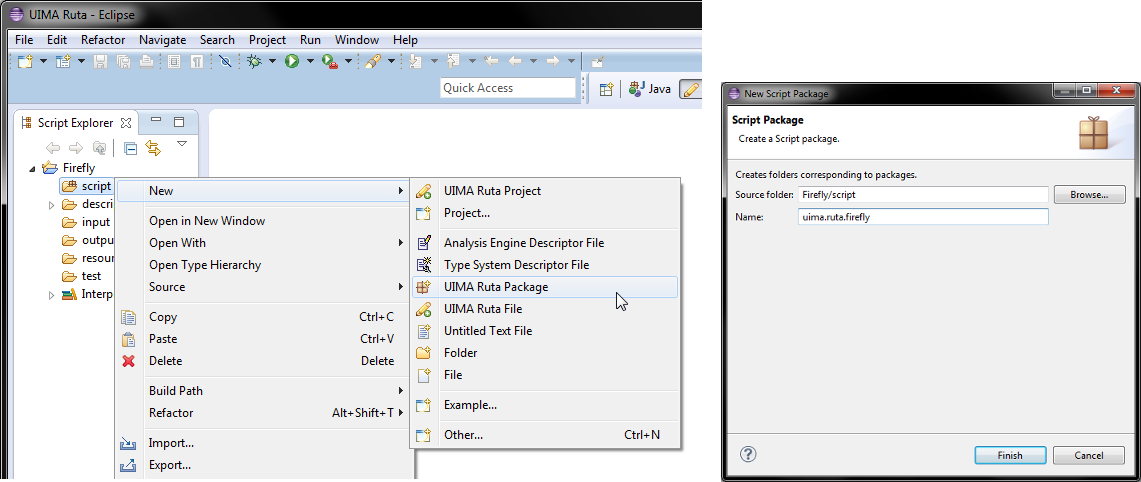
\includegraphics[width=1\textwidth]{figs/capture(7+8).png}
\caption{Ein neues Paket erstellen und einen Namen angeben.}
\label{newpack}
\end{figure}

\begin{figure}
\centering
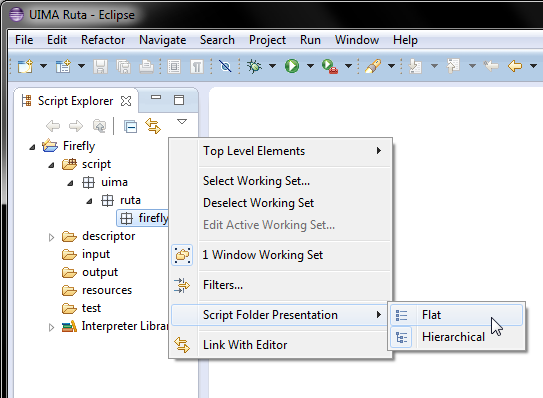
\includegraphics[scale=0.5]{figs/capture(9).png}
\caption{Hierarchische in flache Struktur ändern.}
\label{workbench4}
\end{figure}

\begin{figure}
\centering
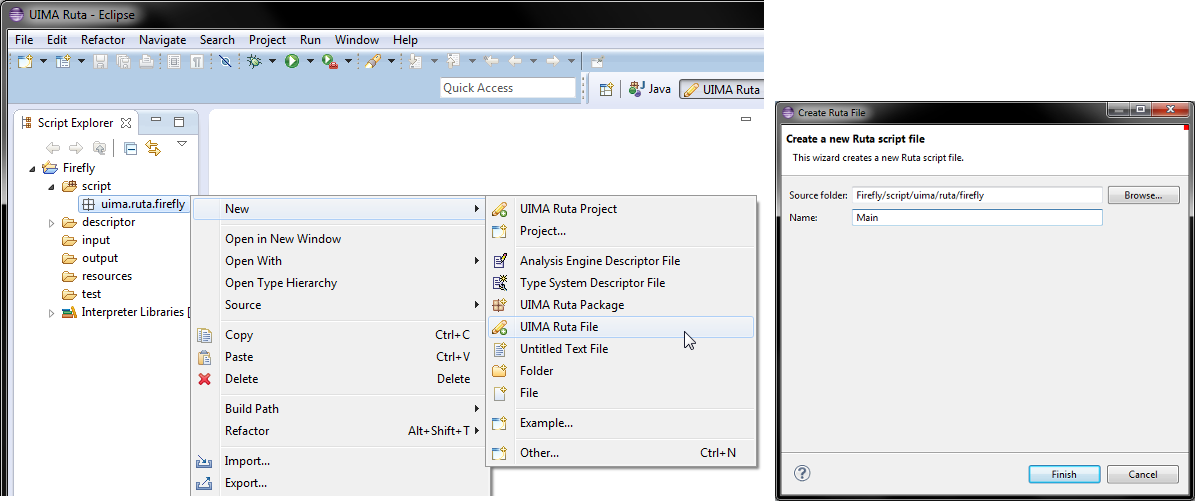
\includegraphics[width=1\textwidth]{figs/capture(10+11).png}
\caption{Ein neues Skript erstellen und einen Namen angeben.}
\label{newscript}
\end{figure}

\newpage
Das waren die ersten Schritte in UIMA Ruta. In Abb.~\ref{workbench5} ist die Arbeitsoberfläche nach erfolgreichem Anlegen aller Dateien. Nun kann mit dem Schreiben der Regeln begonnen werden.

\begin{figure}
\centering
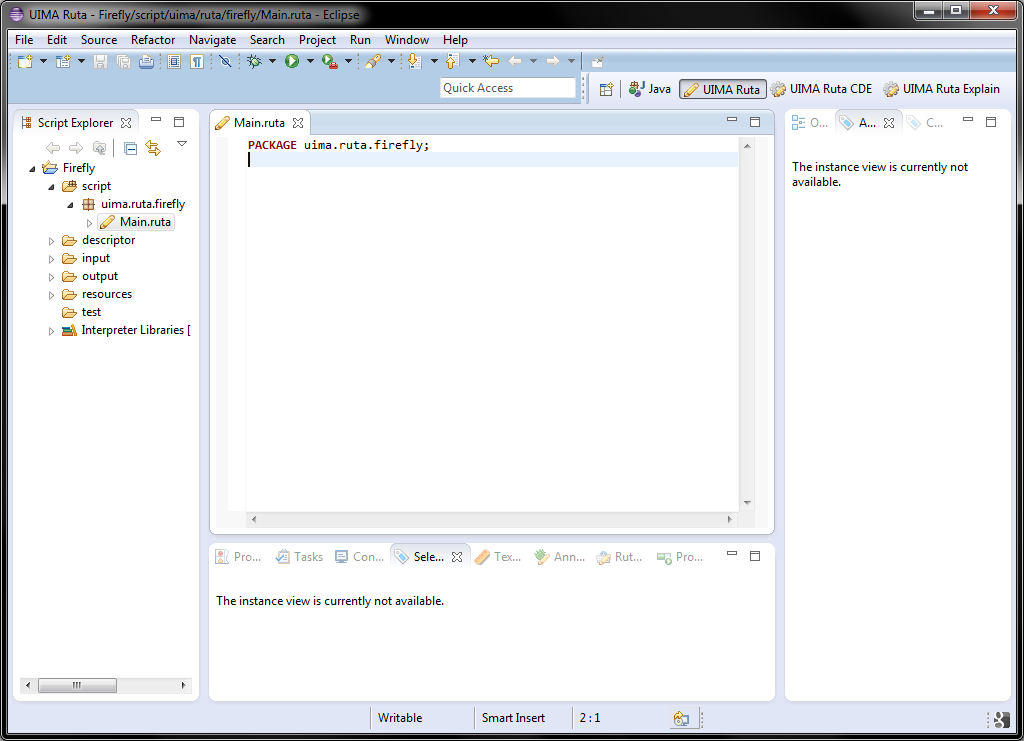
\includegraphics[width=0.5\textwidth]{figs/capture(12).png}
\caption{Die Arbeitsoberfläche nach erfolgreichem Anlegen eines neuen Projekts.}
\label{workbench5}
\end{figure}

\section{Die Sprache UIMA Ruta}\label{lang}
Ein kleines Einstiegsbeispiel soll dabei helfen, die Sprache zu verstehen. Zunächst brauchen wir einen Text, auf dem wir die Regeln entwickeln. Dazu klicken wir auf \textit{input} mit \textbf{Rechtsklick $\rightarrow$ New $\rightarrow$ File} (Abb.~\ref{newdoc}) und wählen im folgenden Fenster einen Namen mit der Endung \glqq .txt\grqq{} für ein Textdokument.

\begin{figure}
\centering
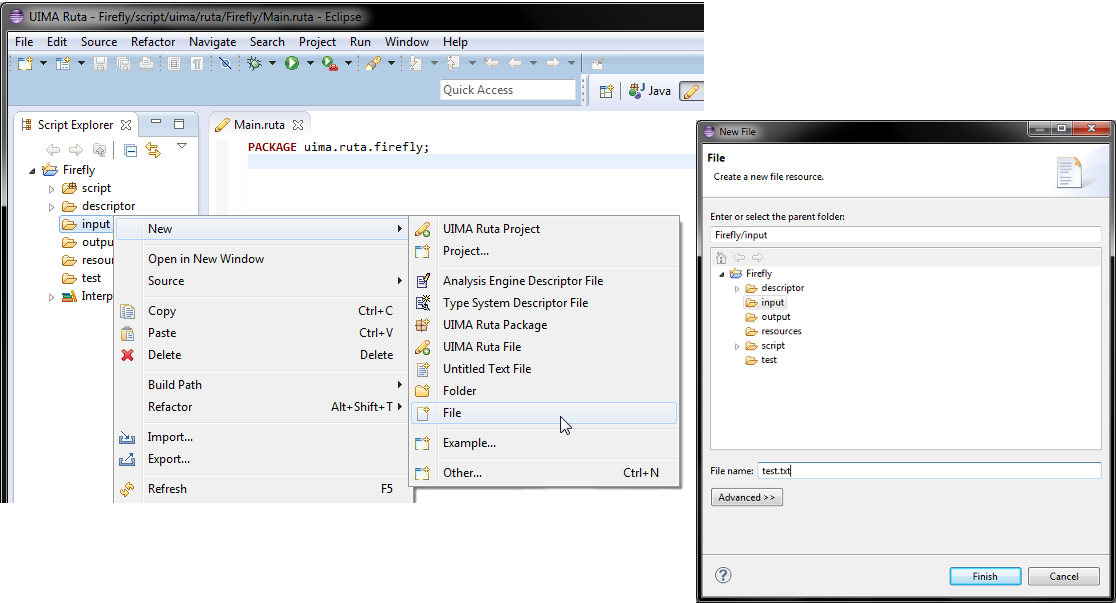
\includegraphics[width=1\textwidth]{figs/capture(13+14).png}
\caption{Ein neues Textdokument erstellen und einen Namen angeben.}
\label{newdoc}
\end{figure}

Danach füllen wir das neu erzeugte Dokument mit einem Text, den wir anschließend mit UIMA Ruta bearbeiten wollen. In Abb.~\ref{text} steht ein Text mit mehreren Personen. Wir wollen versuchen diese Personen zu annotieren.

\begin{figure}
\centering
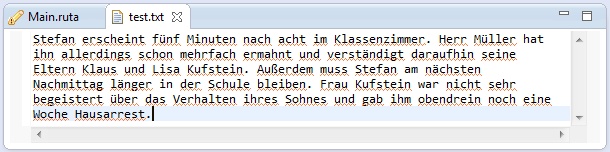
\includegraphics[width=0.75\textwidth]{figs/capture_text.png}
\caption{Beispieltext zum Entwickeln von Regeln.}
\label{text}
\end{figure}

Der erste Schritt der Regelentwicklung ist die Analyse des gegebenen Textes. Ein zentraler Punkt ist, dass in der deutschen Sprache jeder Name großgeschrieben wird. Wir können uns also auf diese Teilmenge der Wörter im Text beschränken. Außerdem fällt im Beispiel auf, dass immer nach \glqq Herr\grqq{} bzw. \glqq Frau\grqq{} ein Nachname steht. Nach dieser Art von Mustern müssen wir also Ausschau halten, wenn wir automatisiert nach Personen suchen wollen. Die  Vornamen im Text sind etwas schwerer ausfindig zu machen. Eine weitere Mög\-lich\-keit in UIMA Ruta ist daher die Verwendung von Wortlisten. \glqq Klaus\grqq{}, \glqq Lisa\grqq{} und \glqq Stefan\grqq{} sind gängige Vornamen. Warum sollte man diese also nicht zur Verwendung in eine Wortliste schreiben?

Die aufgeführten Punkte sind das Gerüst für unsere Regeln. Als erstes wird der Text analysiert und die Ergebnisse notiert. Erst danach überlegt man sich, wie die Informationen umgesetzt werden sollen. In Abb.~\ref{rules} sieht man das Ergebnis unserer Regelumsetzung. Im \textit{Script Explorer} ist jetzt zusätzlich die vom Skript erstellte Ausgabedatei im \textit{output} Ordner. Außerdem wurde \textit{resources} eine Wortliste mit Vornamen hinzugefügt. Auf der rechten Seite ist das Skript.\\
Die Wortlisten sind immer so aufgebaut, dass in jeder Zeile ein Ausdruck stehen muss. Ein Ausdruck ist in unserem Fall ein Vorname. Dies bedeutet aber nicht, dass nur ein Wort pro Zeile stehen darf. Suchen wir beispielsweise den Ort \glqq Frankfurt am Main\grqq, können wir das auch genau so in eine Zeile schreiben. Abb.~\ref{wordlist} zeigt die Wortliste \textit{FirstNames.txt} aus unserem Beispiel. Das Erstellen einer Wortliste ist analog zur Erstellung einer Eingabedatei.

\begin{figure}
\centering
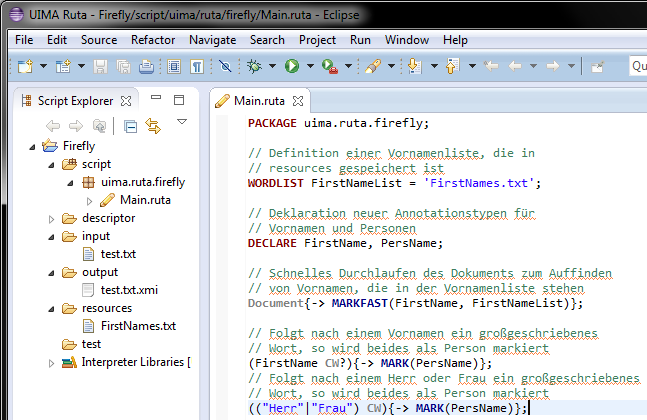
\includegraphics[width=0.75\textwidth]{figs/capture_rules.png}
\caption{Auf der linken Seite ist die vordefinierte Ordnerstruktur mit Inhalt. Auf der rechten Seite ist das Skript mit den Regeln zur Personenfindung im Beispieltext.}
\label{rules}
\end{figure}

\begin{figure}
\centering
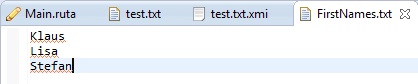
\includegraphics[width=0.5\textwidth]{figs/capture_wordlist.png}
\caption{Zeilenweiser Aufbau der Wortliste mit Vornamen.}
\label{wordlist}
\end{figure}

Wenden wir uns zu den Regeln in Abb.~\ref{rules} und gehen das Skript Zeile für Zeile durch. \texttt{PACKAGE} gibt das Paket des Skriptes an, sodass UIMA Ruta den Speicherort findet. Danach folgen zwei Kommentarzeilen, die mit einem doppelten Slash (\texttt{//}) eingeleitet werden. Ein Kommentar dient der Beschreibung eines Abschnittes in einem Programm bzw. Skript. So kann sich eine zweite Person schnell zurechtfinden, ohne den Code zeilenweise durchgehen zu müssen. Die Wortliste wird mit \texttt{WORDLIST} eingebunden. Vor dem Gleichheitszeichen steht der Variablenname, mit dem wir die Wortliste innerhalb der Regeln ansprechen können. Danach kommt der Dateiname in einfachen Anführungszeichen. Jede Definition, Deklaration oder Regel wird mit einem Strichpunkt (\texttt{;}) beendet. Mit \texttt{DECLARE} definieren wir neue Annotationstypen \textit{FirstName} und \textit{PersName}. Alle vordefinierten Annotationstypen sind in Abb.~\ref{tokens} abgebildet und werden von UIMA Ruta selbst erzeugt.

\begin{figure}
\centering
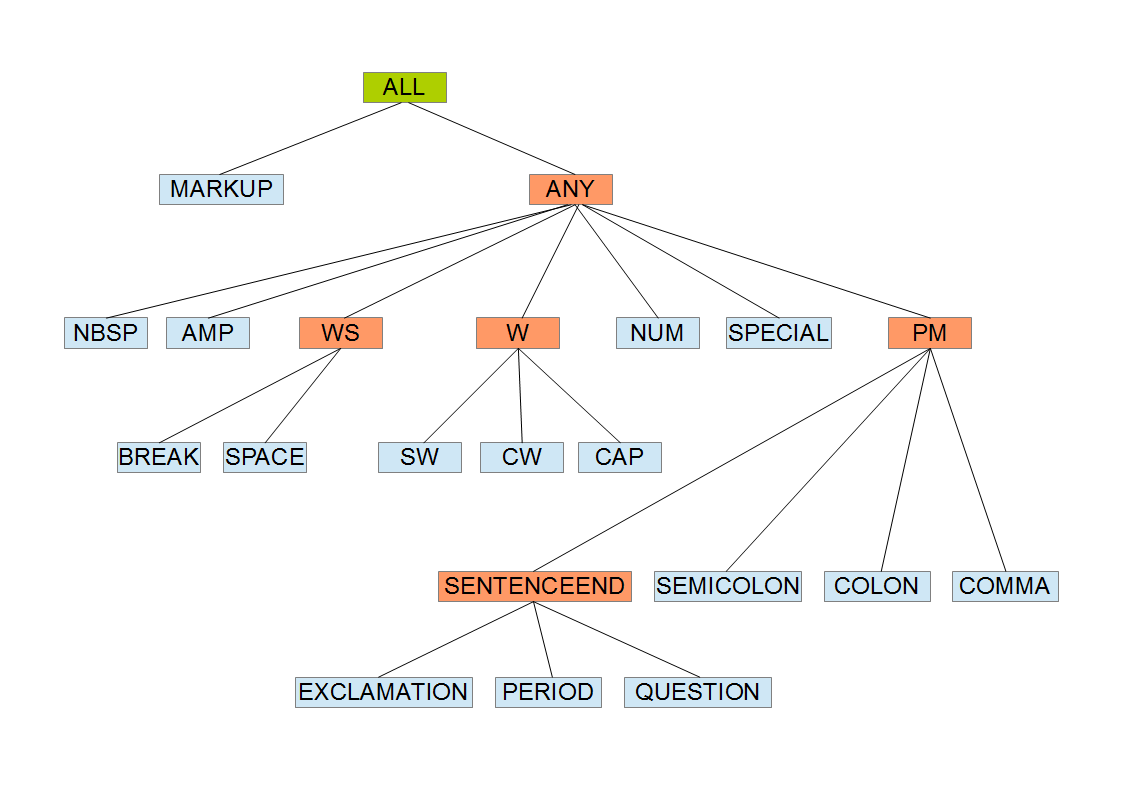
\includegraphics[width=0.75\textwidth]{figs/basic_token.png}
\caption{Sämtliche Klassen von Tokens von UIMA Ruta.}
\label{tokens}
\end{figure}

Unsere Deklarationen werden erst im Skript erzeugt, indem wir einen gefundenen Abschnitt markieren. Eine Option wäre \texttt{MARKFAST}. Dazu muss zunächst mit \texttt{Document} das aktuelle Dokument angesprochen werden. Jetzt folgt die Aktion in geschweiften Klammern (\texttt{$\{\}$}) und einem Pfeil nach rechts (\texttt{->}). Die Aktion \texttt{MARKFAST} nimmt dann zwei Parameter entgegen. Der Erste ist der Annotationstyp, den wir annotieren wollen. Der zweite Parameter ist die Wortliste, mit der wir das Dokument abgleichen. Anschließend wird das gesamte Dokument auf die Zeilen in der Wortliste geprüft. Jeder Treffer wird als \textit{FirstName} markiert und ist als solcher in den Regeln verfügbar. Eine andere Option ist \texttt{MARK}. Die Aktion \texttt{MARK} hat meistens einen Parameter. Dieser ist der Annotationstyp mit dem wir einen bestimmten Abschnitt annotieren wollen, hier als \textit{PersName}. Der Ausdruck vor der geschweiften Klammer steht in runden Klammern (\texttt{()}). Somit wird jeder Abschnitt, der den Regeln innerhalb der Klammern entspricht, als \textit{PersName} markiert. Die Regel \texttt{FirstName CW?} sucht nach einem \textit{FirstName} und prüft dann, ob ein großgeschriebenes Wort (CW = capitalized word) folgt. Ist dies der Fall, wird beides als \textit{PersName} markiert. Ein Treffer in unserem Text ist also \glqq Lisa Kufstein\grqq{}, da \glqq Lisa\grqq{} zuvor als \textit{FirstName} markiert wurde und \glqq Kufstein\grqq{} ein großgeschriebenes Wort ist. Das Fragezeichen (\texttt{?}) ist ein Quantifizierer, der die Optionalität von \texttt{CW} ausdrückt. Deswegen wird auch \glqq Stefan\grqq{} und \glqq Klaus\grqq{} als \textit{PersName} markiert. Die letzte Regel \texttt{("Herr"$\mid$"Frau") CW} sucht nach dem Ausdruck \glqq Herr\grqq{} oder \glqq Frau\grqq{}. Folgt darauf ein großgeschriebenes Wort, wird es als \textit{PersName} markiert. Diese Regel findet \glqq Herr Müller\grqq{} und \glqq Frau Kufstein\grqq{} in unserem Beispiel. Wir starten das Skript, indem wir den grünen Kreis mit dem Pfeil unterhalb der Menüleiste drücken. Mit einem Doppelklick auf die Datei im \textit{output} Ordner lässt sie sich einsehen. Sollte UIMA Ruta nach einem geeigneten Typesystem fragen (Abb.~\ref{typesystem}), sucht ihr den Namen eures Skripts mit angehängtem \glqq TypeSystem.xml\grqq{}.

\begin{figure}
\centering
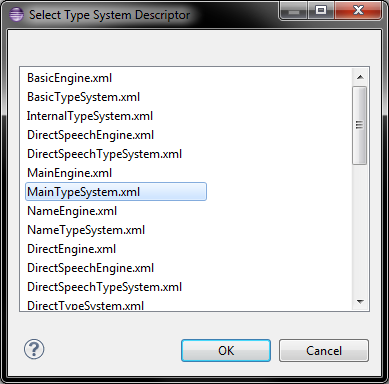
\includegraphics[width=0.5\textwidth]{figs/typesystem.png}
\caption{Auswahlfenster für ein Typesystem.}
\label{typesystem}
\end{figure}

Das Ergebnis unserer Entwicklung ist in Abb.~\ref{marked} zu sehen. Auf der linken Seite ist der markierte Text, während auf der rechten Seite im \textit{Annotation Browser View} jede Annotation des angezeigten Textes ausgewählt werden kann.

\begin{figure}
\centering
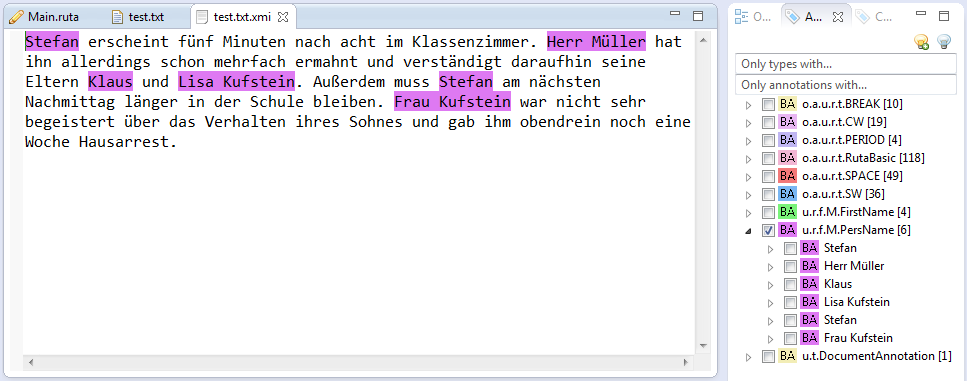
\includegraphics[width=0.75\textwidth]{figs/capture_marked.png}
\caption{Auf der linken Seite ist der markierte Text. Rechts im \textit{Annotation Browser View} können Annoationstypen ausgewählt werden, die im Text markiert werden sollen}
\label{marked}
\end{figure}

Jeder Annotationstyp wird in einer eindeutigen Farbe hervorgehoben. Mit dem angefertigten Skript haben wir jede Person in dem Beispieltext gefunden. Im nächsten Kapitel wenden wir uns dem literarischen Text zu. Eine vollständige Auflistung und Erklärung aller Spracheigenschaften von UIMA Ruta ist im \textit{Apache UIMA{\texttrademark} Ruta Guide and Reference}\footnote{\url{https://uima.apache.org/d/ruta-current/tools.ruta.book.html}}.

\section{Personenfindung in \glqq Der Idiot\grqq}
Das Wissen aus Kapitel~\ref{lang} wollen wir nun auf das erste Kapitel von Dostojewskis \glqq Der Idiot\grqq anwenden. Es werden fortgeschrittene Regeln verwendet, die u.a. nicht auf die Technik des \textit{Part-of-speech Tagging} verzichten können. Dabei wird jedes Wort und Satzzeichen einer Wortart (part of speech) zugeordnet. Es werden sowohl Wortdefinitionen, als auch der Kontext zur Analyse herangezogen. Der in Kapitel~\ref{tt} vorgestellte TreeTagger ist ein solches Analysewerkzeug, den wir für unser Beispiel in UIMA Ruta einbinden werden.

\subsection{Einbindung von TreeTagger}
Als erstes muss das Projekt \textit{Firefly} konvertiert werden. Dazu klicken wir auf das Projekt mit \textbf{Rechtsklick $\rightarrow$ Configure $\rightarrow$ Convert to Maven Project}, wie in Abb.~\ref{convert} dargestellt. Im darauffolgenden Fenster wird mit \textit{Finish} ein neues \textit{pom.xml} erstellt. Ist der Eintrag \textit{Convert to Maven Project} nicht verfügbar, fehlt das entsprechende Paket. Zur Installation des Paketes gehen wir zu \textbf{Help $\rightarrow$ Install New Software...} und wählen unter \textit{Work with} alle eingetragenen Seiten aus (Abb.~\ref{m2e_install}). Anschließend suchen wir das Paket \textit{m2e - Maven Integration for Eclipse} unter dem Punkt \textit{Collaboration}. Die Installation startet, nachdem wir zweimal auf \textit{Next} drücken und den Lizenzbedingungen zustimmen. Falls während der Installation ein Fenster erscheint, das uns vor unsigniertem Inhalt warnt, wird es einfach mit \textit{OK} bestätigt.

\begin{figure}
\centering
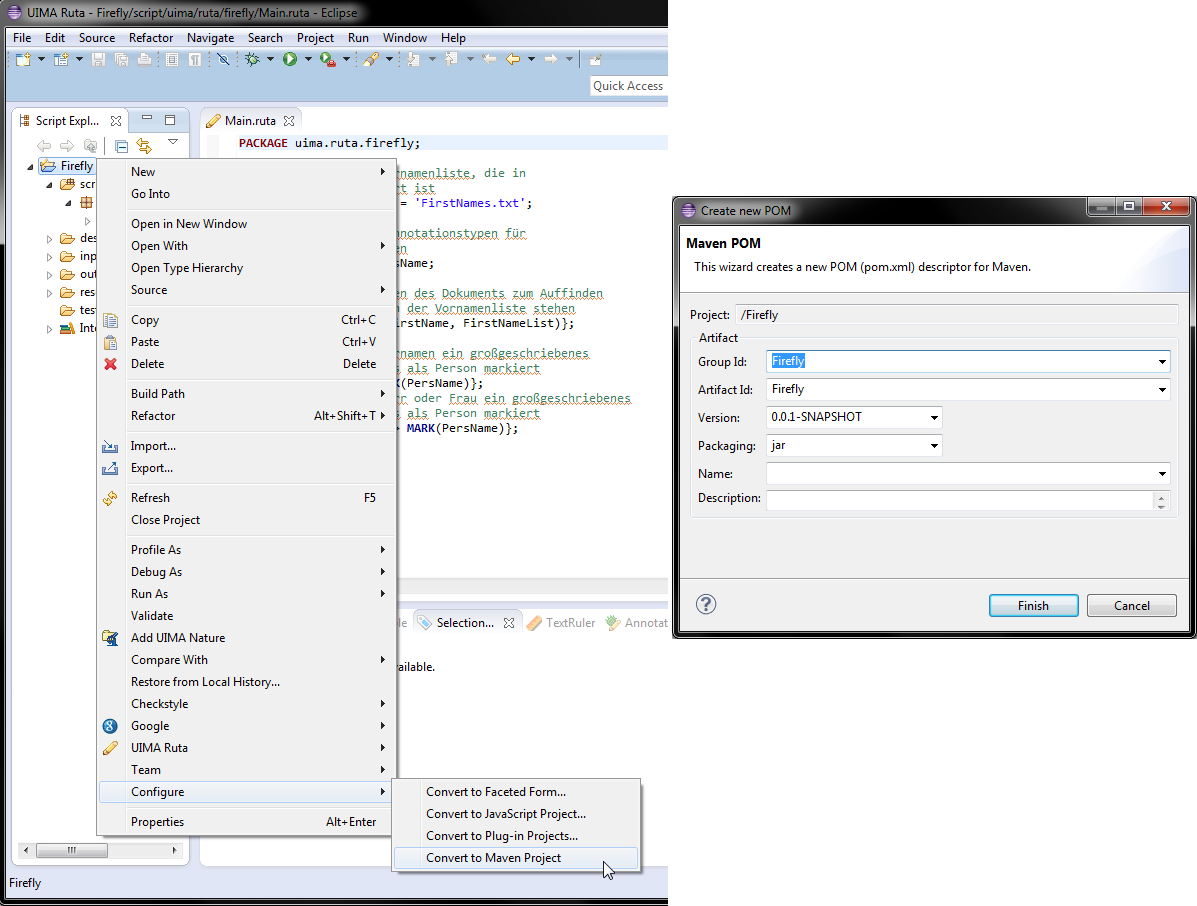
\includegraphics[width=0.75\textwidth]{figs/tt_convert.png}
\caption{Das UIMA Ruta Projekt wird in ein Maven Projekt konvertiert.}
\label{convert}
\end{figure}

\begin{figure}
\centering
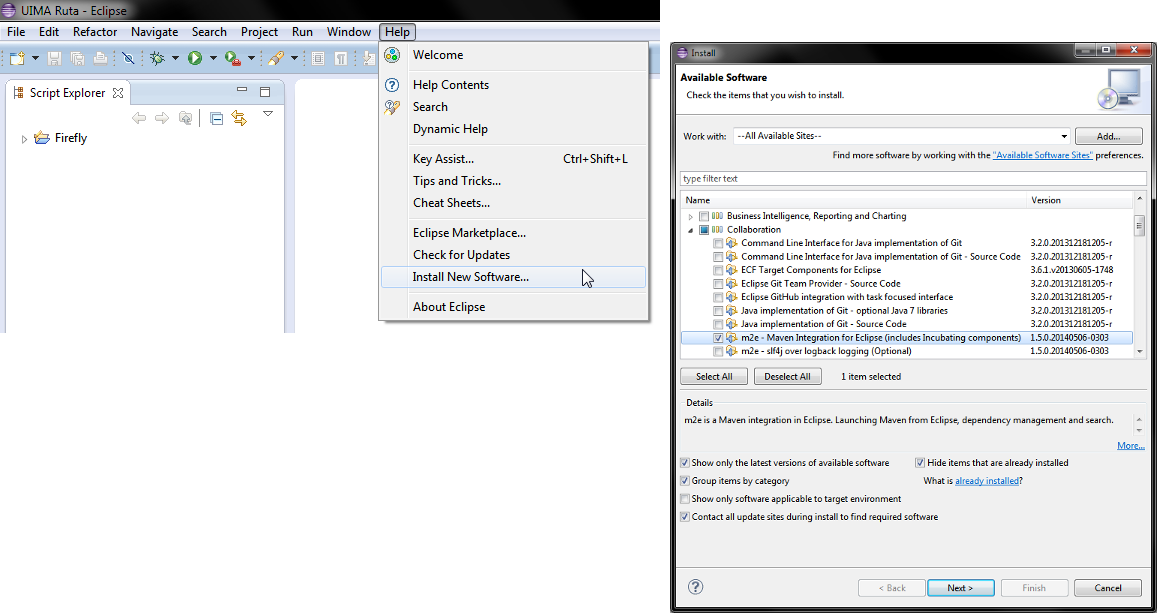
\includegraphics[width=1\textwidth]{figs/m2e_install.png}
\caption{Im Menü \textit{Help} wird die Softwareinstallation ausgewählt. Anschließend müssen die entsprechenden Pakete zur Installation ausgewählt werden.}
\label{m2e_install}
\end{figure}

Ist die Datei \textit{pom.xml} erstellt, öffnet sie sich sofort in der Übersicht (Abb.~\ref{overview}). Wir navigieren unten von \textit{Overview} nach \textit{pom.xml}, um den Inhalt der Datei zu bearbeiten (Abb.~\ref{pom}).

\begin{figure}
\centering
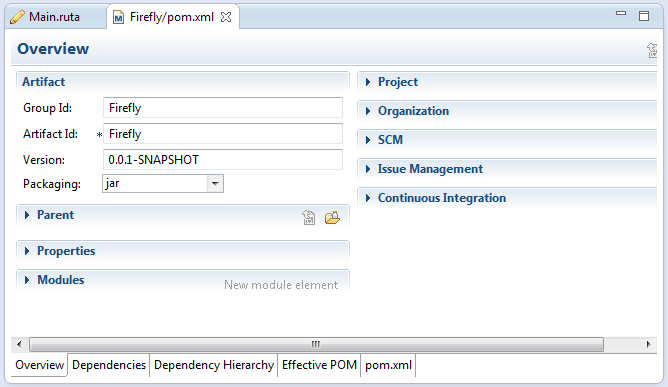
\includegraphics[width=0.5\textwidth]{figs/tt_overview.png}
\caption{Übersicht der POM-Datei.}
\label{overview}
\end{figure}

\begin{figure}
\centering
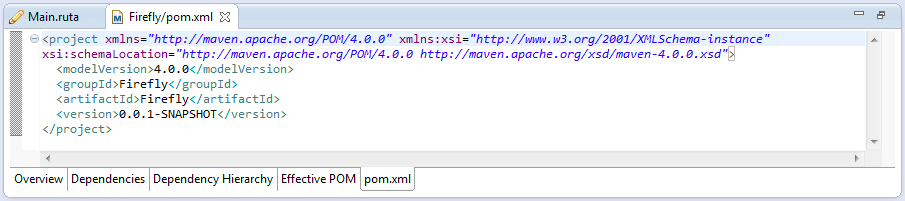
\includegraphics[width=1\textwidth]{figs/tt_pom.png}
\caption{Der Inhalt von \textit{pom.xml} nach der Konvertierung.}
\label{pom}
\end{figure}

\newpage

Vor dem Eintrag \texttt{</project>} muss zur Einbdinung von TreeTagger folgender Text eingefügt werden:

\begin{center}
\begin{lstlisting}[language=XML,
frame=L,
stepnumber=0,
basicstyle=\scriptsize\ttfamily,
morekeywords={parent,groupId,artifactId,dependencies,dependency,
repositories,repository,id,url,snapshots, enabled},
keywordstyle=\color{mygreen},
keepspaces=true]
<parent>
  <groupId>org.apache.uima</groupId>
  <artifactId>ruta-parent</artifactId>
  <version>2.1.0</version>
</parent>
<dependencies>
  <dependency>
    <groupId>de.tudarmstadt.ukp.dkpro.core</groupId>
    <artifactId>de.tudarmstadt.ukp.dkpro.core.treetagger-asl</artifactId>
    <version>1.5.0</version>
  </dependency>
  <dependency>
    <groupId>de.tudarmstadt.ukp.dkpro.core</groupId>
    <artifactId>de.tudarmstadt.ukp.dkpro.core.stanfordnlp-gpl</artifactId>
    <version>1.5.0</version>
  </dependency>
</dependencies>
<repositories>
  <repository>
    <id>ukp-oss-model-releases</id>
    <url>
      http://zoidberg.ukp.informatik.tu-darmstadt.de/
      artifactory/public-model-releases-local
    </url>
    <snapshots>
      <enabled>false</enabled>
    </snapshots>
  </repository>
</repositories>
\end{lstlisting}
\end{center}

Das Ergebnis ist in Abb.~\ref{pom2} zu sehen.

\begin{figure}
\centering
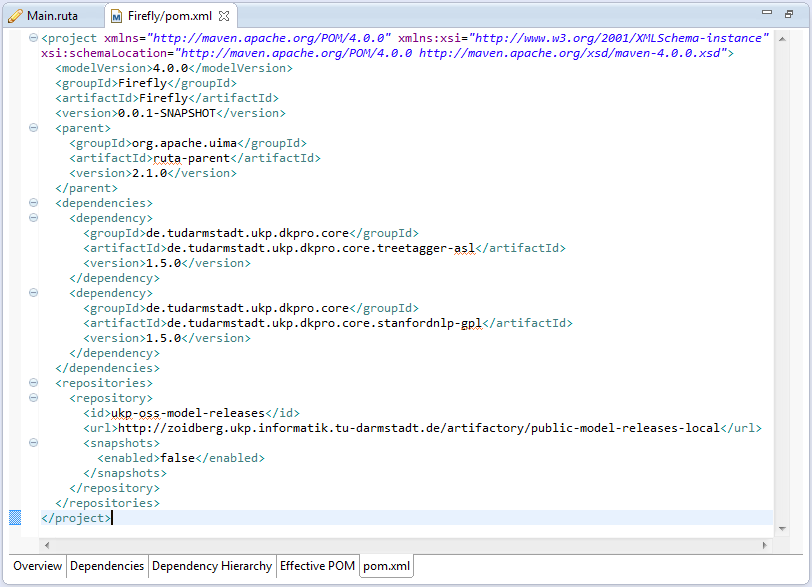
\includegraphics[width=0.75\textwidth]{figs/tt_pom2.png}
\caption{Der Inhalt des \textit{pom.xml} nach Einfügen der Abhängigkeiten.}
\label{pom2}
\end{figure}

Nachdem das \textit{pom.xml} bearbeitet wurde, müssen wir das Projekt updaten. Dazu klicken wir auf das Projekt und drücken \textbf{Alt + F5}. Darauf erscheint ein Fenster zum Aktualisieren des Projektes (Abb.~\ref{update}), das wir einfach mit \textit{OK} bestätigen.

\begin{figure}
\centering
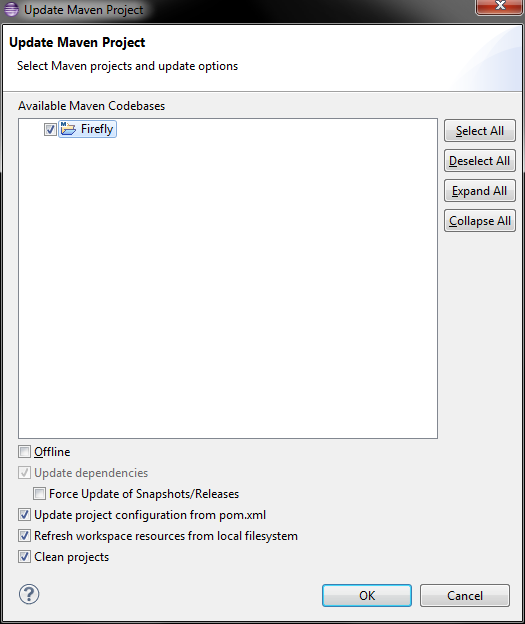
\includegraphics[width=0.5\textwidth]{figs/tt_maven.png}
\caption{Fenster zum Aktualisieren eines Maven Projektes.}
\label{update}
\end{figure}

Sollte nun unter \textit{Problems} der Fehler aus Abb.~\ref{error} vorhanden sein, beheben wir ihn mit der Schnellhilfe. Dazu klicken wir auf den Eintrag mit \textbf{Rechtsklick $\rightarrow$ Quick Fix} und bestätigen das nächste Fenster mit \textit{Finish}.

\begin{figure}
\centering
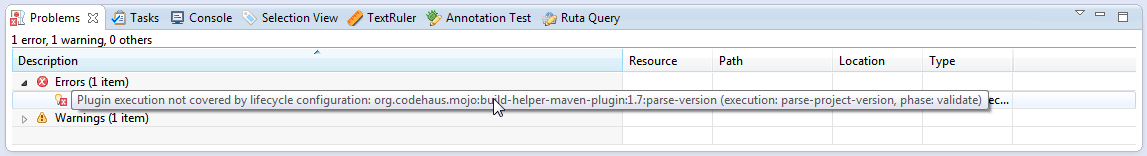
\includegraphics[width=1\textwidth]{figs/maven_error.png}
\caption{Möglicher Fehler nach der Projektkonvertierung.}
\label{error}
\end{figure}

Anschließend öffnet sich der \textit{m2e Marketplace} (Abb.~\ref{marketplace}), den wir ebenfalls mit einem \textit{Finish} bestätigen. Wir folgen den Schritten zur Installation des \textit{buildhelper}, nach denen der Fehler behoben sein sollte.

Der nächste Schritt fügt das Typesystem von TreeTagger hinzu. Dazu kopieren wir die  Datei \textit{GeneratedDKProCoreTypes.xml} aus dem Anhang in den Ordner \textit{descriptor}. Anschließend sollte der \textit{Script Explorer} wie in Abb.~\ref{dkpro} aussehen.

\begin{figure}
\centering
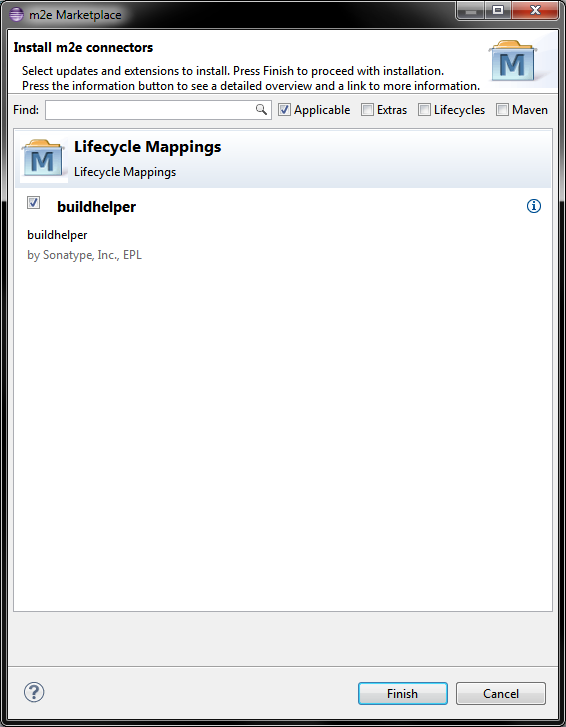
\includegraphics[width=0.5\textwidth]{figs/maven_marketplace.png}
\caption{Der \textit{m2e Marketplace}.}
\label{marketplace}
\end{figure}

\begin{figure}
\centering
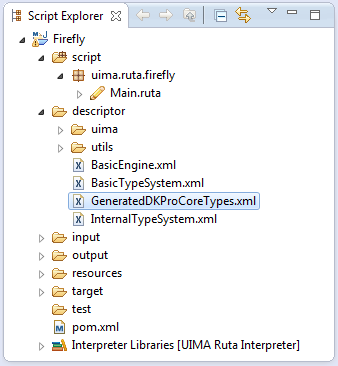
\includegraphics[width=0.5\textwidth]{figs/tt_dkpro.png}
\caption{Das Typesystem DKPro in \textit{descriptor} kopieren.}
\label{dkpro}
\end{figure}

Nun kann TreeTagger in UIMA Ruta verwendet werden. Als letzten Schritt erzeugen wir, wie in Kapitel~\ref{first_project} beschrieben, ein neues Paket und Skript. Dieses Skript ruft den Part-of-speech Tagger auf und versieht das Eingabedokument mit neuen Annotationstypen. Jetzt kann es in \textit{Main.ruta} aufgerufen werden, damit wir die Annotationstypen in unseren Regeln nutzen können. Der Inhalt des neuen Skripts ist in Abb.~\ref{pos} zu sehen.

\begin{figure}
\centering
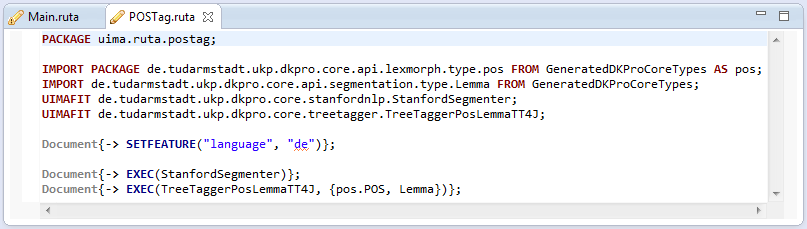
\includegraphics[width=1\textwidth]{figs/tt_pos.png}
\caption{Ein Skript zum Ausführen des TreeTaggers.}
\label{pos}
\end{figure}

Führt man das Skript auf dem Eingabetext aus, können im \textit{Annotation Browser View} weitere Annotationstypen ausgewählt werden (Abb.~\ref{pos2}).

\begin{figure}
\centering
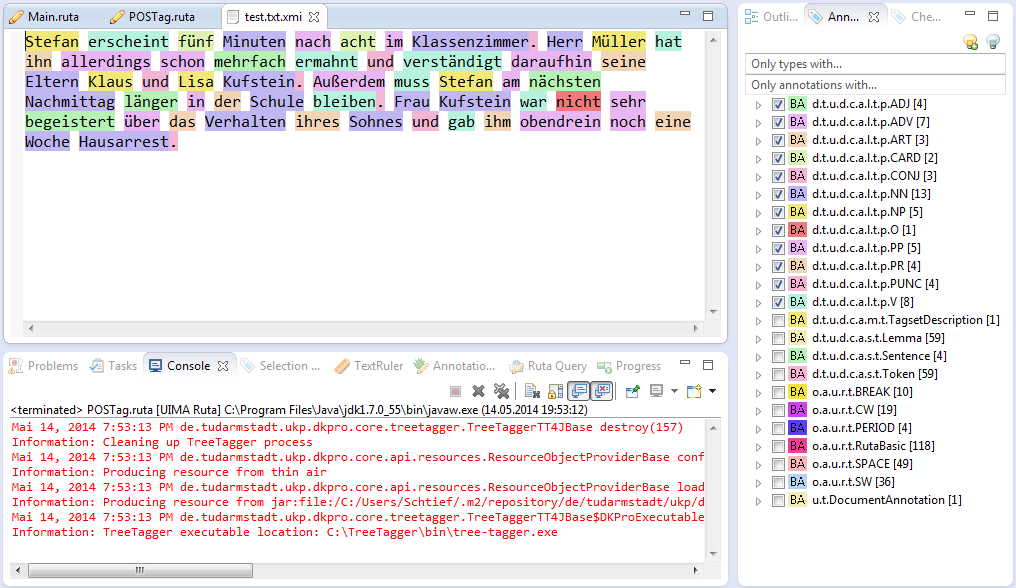
\includegraphics[width=0.75\textwidth]{figs/tt_pos2.png}
\caption{Im \textit{Annotation Browser View} sind alle Annotationstypen von TreeTagger ausgewählt. Für jedes Wort gibt es links eine spezielle Zuordnung.}
\label{pos2}
\end{figure}

\subsection{Weiterentwicklung der Regeln}
Das Projekt wird immer größer, also ist es ratsam, möglichst jede Aufgabe aufzuteilen. Das bedeutet, wir haben ein Skript für die Annotationstypen von TreeTagger, ein Skript für das Finden von Namen im Text und ein anderes, das alle Skripte aufruft und somit das Hauptskript wird. Jetzt kann jeder Teilbereich getestet werden, ohne, dass wir jedes Skript ausführen müssen. Das Hauptskript wird \textit{Main.ruta} sein (Abb.~\ref{main}) und alle anderen relevanten Skripte aufrufen. Der Befehl \texttt{SCRIPT} importiert ein Skript, während es der Befehl \texttt{CALL} ausführt. Die zwei Zeilen vor dem Skriptimport müssen in jedes Skript eingefügt werden, das TreeTagger nutzt.

\begin{figure}
\centering
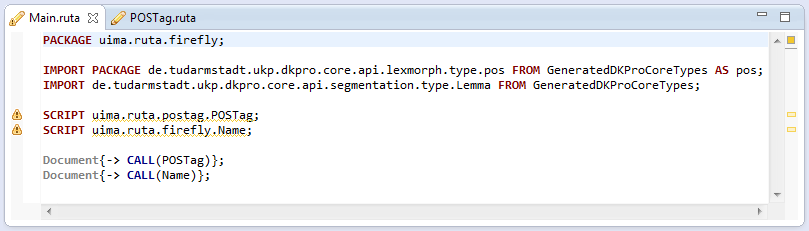
\includegraphics[width=1\textwidth]{figs/tt_main.png}
\caption{Das Hauptskript, indem alle Skripte aufgerufen und ausgeführt werden.}
\label{main}
\end{figure}

Die bisher entwickelten Regeln kopieren wir in das Skript \textit{Name.ruta}, wie in Abb.~\ref{name} zu sehen ist. Dabei ist wieder zu beachten, dass die zwei Zeilen im Kopfteil eingefügt werden.

\begin{figure}
\centering
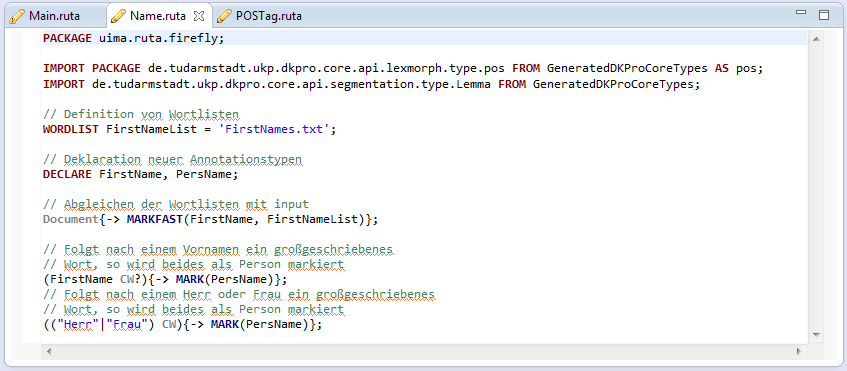
\includegraphics[width=1\textwidth]{figs/tt_name.png}
\caption{Der ursprüngliche Inhalt des Hauptskriptes wird in \textit{Name.ruta} kopiert.}
\label{name}
\end{figure}

Der erste Schritt für unser neues Dokument ist wieder die Textanalyse. Zunächst kopieren wir aber das beigefügte Dokument \textit{dostoevskij - idiot.txt} in den \textit{input} Ordner und löschen die Datei \textit{test.txt} aus \textit{input} und \textit{output}. Durch Doppelklicken öffnen wir das Textdokument und beginnen mit der Analyse. Währenddessen können die Vornamen, die noch nicht in unserer Liste stehen, hinzugefügt werden. Es fällt auf, dass häufig direkte Reden verwendet werden. Vor einer direkten Rede, bzw. danach, ist der Sprecher oft erwähnt. Weiter fällt auf, dass ein Titel, wie \glqq Herr\grqq{}, und ein folgendes großgeschriebenes Wort auf eine Person hindeutet. Ein Titel ist dabei ganz allgemein gehalten oder kann eine Berufsbezeichnung, Adelstitel oder Familienzugehörigkeit sein. Mit diesen Informationen können einfache Regeln realisiert werden. Wie für die Vornamen brauchen wir auch für alle Titel eine Wortliste. Dazu legen wir ein paar neue Wortlisten in \textit{resources} an, wie es in Kapitel~\ref{first_project} beschrieben wurde. Alle Titel sollten alphabetisch geordnet sein, damit ein weiteres Hinzufügen von Titeln nicht zu Problemen führt. Zum Schluss haben wir jeweils eine Liste für Berufe, Adelstitel, Angehörige und Militärgrad. Die Titel bzw. Vornamen werden manuell eingefügt oder können aus einer Internetdatenbank heruntergeladen werden. Ein Ausschnitt der Wortlisten ist in Abb.~\ref{titles} zu sehen.

\begin{figure}
\centering
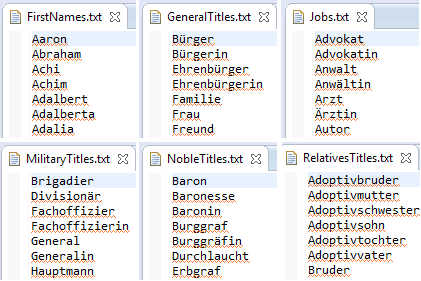
\includegraphics[width=0.6\textwidth]{figs/tt_titles.png}
\caption{Ausschnitt der verschiedenen Wortlisten.}
\label{titles}
\end{figure}

Als nächstes müssen nur noch die Regeln angepasst und erweitert werden. Dazu zählen die neuen Wortlisten, neue Deklarationen für die Titel und das Durchlaufen des Dokuments mit \texttt{MARKFAST}. Die Änderungen und die neuen Regeln sind in Abb.~\ref{name2} zu sehen. Zur besseren Verständlichkeit ist jeder Regelabschnitt mit einem großgeschriebenen Kommentar als Überschrift gekennzeichnet.

\begin{figure}
\centering
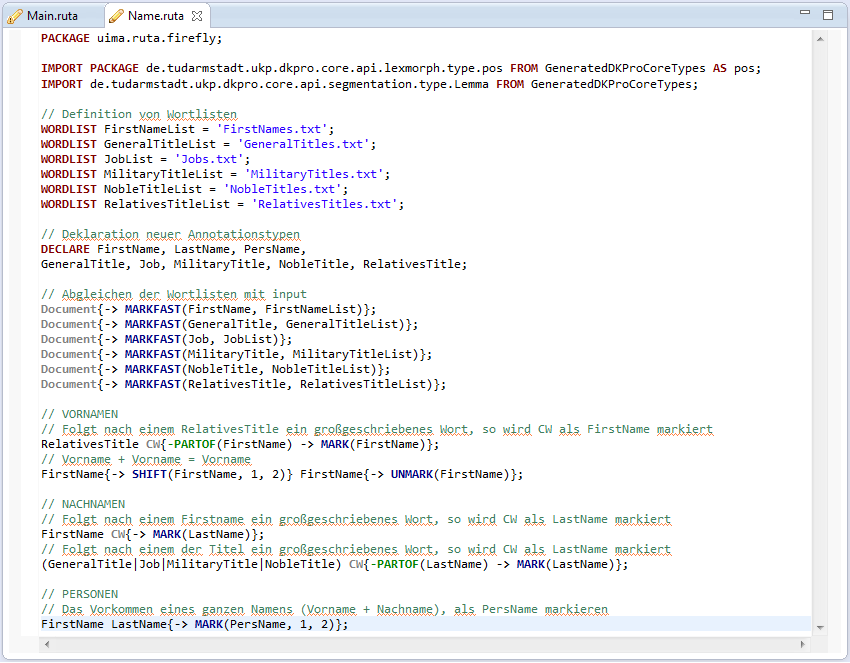
\includegraphics[width=1\textwidth]{figs/tt_name2.png}
\caption{Die neuen Wortlisten werden eingefügt und die Regeln erweitert.}
\label{name2}
\end{figure}

Die erste Regel im Vornamenabschnitt sucht nach Titeln, die zuvor als \textit{RelativesTitle} markiert wurden. Folgt danach ein großgeschriebenes Wort, ist dies ein potenzieller Vorname und wird als \textit{FirstName} markiert. Der \texttt{-PARTOF} Befehl verhindert, dass ein schon annotierter \textit{FirstName} doppelt markiert wird. Die zweite Regel findet einen \textit{FirstName} gefolgt von einem \textit{FirstName}. In \glqq Der Idiot\grqq{} hat fast jede Person einen zweiten Vornamen. Diese Vorkommen wollen wir finden und beide Vornamen zu einem einzigen \textit{FirstName} verbinden. \texttt{SHIFT} weitet dabei die Annotation des ersten \textit{FirstName} auf das zweiten \textit{FirstName} aus. Jetzt ist der zweite Vorname allerdings doppelt markiert und muss mit \texttt{UNMARK} wieder demarkiert werden. Im Nachnamenabschnitt suchen wir zunächst nach Vornamen mit einem angehängten, großgeschriebenen Wort. Trifft die Regel auf einen Abschnitt zu, wird das letzte Wort als \textit{LastName} markiert. Mit der zweiten Regel suchen wir Personen, wie \glqq Generalin Jepantschina\grqq{}. Folgt \texttt{CW} auf ein \textit{MilitaryTitle} o.ä., wird das letzte Wort als \textit{LastName} markiert. Dies geschieht wiederum nur, wenn das gefundene \texttt{CW} noch kein \textit{LastName} ist (\texttt{-PARTOF}). Im letzten Abschnitt verbinden wir nun die \textit{FirstName} und \textit{LastName} zu einer Person als \textit{PersName}. \texttt{MARK(PersName, 1, 2)} weitet die Annotation auf das erste und zweite Element in der Regel aus. Das Ergebnis unserer Entwicklung ist in Abb.~\ref{ano} zu sehen.

\begin{figure}
\centering
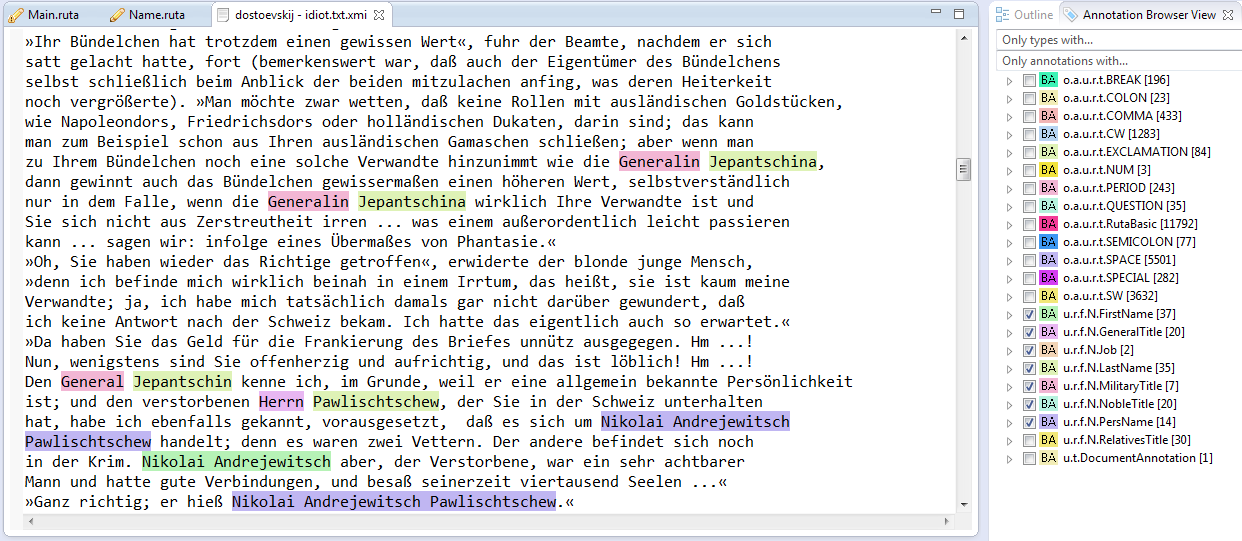
\includegraphics[width=1\textwidth]{figs/tt_ano.png}
\caption{Das Ergebnis der Erweiterungen links im Fenster. Personen werden teilweise vollständig erkannt.}
\label{ano}
\end{figure}

Für den Ansatz, mit direkter Rede auf eine Person zu schließen, erstellen wir ein neues Skript. Darin befinden sich sämtliche Regeln, die eine direkte Rede erkennen und als \textit{DirectSpeech} markieren (Abb.~\ref{speech}). Das Zeichen \texttt{\#} stellt den gesamten Inhalt zwischen dem ersten und letzten Zeichen der Regel dar. Dies wäre also die gesamte Aussage einer Person. \texttt{MARK(DirectSpeech, 1, 2, 3)} markiert anschließend den gesamten Abschnitt als \textit{DirectSpeech}.

\begin{figure}
\centering
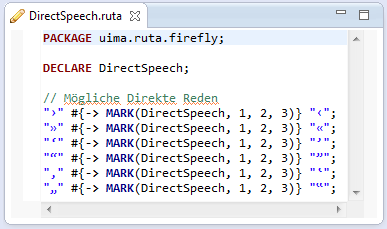
\includegraphics[width=0.5\textwidth]{figs/tt_speech.png}
\caption{Das Skript zum Erkennen direkter Rede.}
\label{speech}
\end{figure}

Anschließend importieren wir das Skript mit \texttt{SCRIPT} in \textit{Name.ruta} und füh\-ren es mit \texttt{CALL} aus. Für die Regel ist nun der zuvor eingerichtete TreeTagger notwendig. Mit diesem können wir nicht nur kleine und große Wörter erkennen, sondern sie auch einer Wortart zuordnen. Zusätzlich benötigen wir noch eine Liste mit Verben, die eine direkte Rede einleiten bzw. beenden. Dies wären beispielsweise Wörter wie \glqq sagen\grqq{} oder \glqq antworten\grqq{}. Die Liste sollte als Wortliste definiert, aber nicht mit \texttt{MARKFAST} ausgeführt werden. Die Regel aus Abb.~\ref{speech2} wird dann am Ende des Personenabschnittes eingefügt. Diese markiert den Sprecher nach einer direkten Rede als \textit{PersName}.

\begin{figure}
\centering
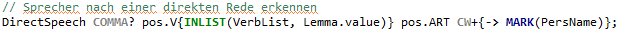
\includegraphics[width=0.9\textwidth]{figs/tt_speech2.png}
\caption{Die Regel, um Sprecher nach einer direkten Rede zu erkennen.}
\label{speech2}
\end{figure}

Die Annotationstypen, die mit \glqq pos.\grqq{} eingeleitet werden, sind von TreeTagger und reichen von Nomen und Verben, bis zu Personal- und Reflexivpronomen. Der gesamte Umfang der Annotationstypen des Part-of-speech Taggers ist in der entsprechenden Dokumentation\footnote{\url{http://www.cis.uni-muenchen.de/~schmid/tools/TreeTagger/data/stts_guide.pdf}} zu finden. Zunächst sucht UIMA Ruta nach einer direkten Rede und einem optionalen Komma. Danach muss ein Verb aus unserer Wortliste stehen. \texttt{INLIST} gleicht das Verb mit der Wortliste ab. Das Besondere dabei ist, dass der \textit{Lemma.value} des gefundenen Wortes überprüft wird, nicht das Verb selbst. Somit steht in unserer Wortliste nur die Grundform eines Verbs, z.B. \glqq sagen\grqq{}, und nicht jede Deklination, z.B. \glqq sagte\grqq{}. Der \textit{Lemma.value} eines Wortes ist also die Grundform. Jedes \textit{Lemma.value} kann im \textit{Selection View} eines geöffneten Dokumentes eingesehen werden, das mit dem TreeTagger bearbeitet wurde. Nach dem Verb folgt ein Artikel mit dem großgeschriebenen Wort. Das \texttt{CW} ist unsere gefundene Person und wird als \textit{PersName} annotiert. Das Plus (\texttt{+}) ist ein Quantifizierer und drückt aus, dass mindestens ein \texttt{CW} folgt. Die Regel findet sowohl \glqq Schwarzhaarige\grqq{}, als auch \glqq Schweizer Patient\grqq{}.

\section{Der Annotation Test}
Der \textit{Annotation Test} hilft uns dabei, unsere Regeln automatisch zu evaluieren. Bei sehr großen oder vielen Texten ist es nur sehr aufwendig, das Ergebnis manuell zu überprüfen. Der \textit{Annotation Test} hingegen liefert uns einen genauen Überblick über unsere Trefferquote.

\subsection{Das Referenzdokument}

Damit der Test überhaupt durchgeführt werden kann, benötigen wir ein Referenzdokument. In diesem Dokument müssen alle Annotationen vorhanden sein, die wir mit unserem Skript finden wollen. Bei der späteren Bearbeitung dieses Dokumentes müssen die entsprechenden Annotationstypen in der XMI-Datei vorhanden sein. Neue Annotationstypen können nicht erstellt werden. Deswegen starten wir das Skript \textit{Main.ruta} und kopieren das Ausgabedokument aus \textit{output} in den Unterordner \textit{test $\rightarrow$ uima $\rightarrow$ ruta $\rightarrow$ firefly $\rightarrow$ Name}. Anschließend wählen wir das Skript \textit{Name.ruta} an und klicken auf den Reiter \textit{Annotation Test}. Die Arbeitsoberfläche sollte jetzt ähnlich der Abb.~\ref{test_main} sein.

\begin{figure}
\centering
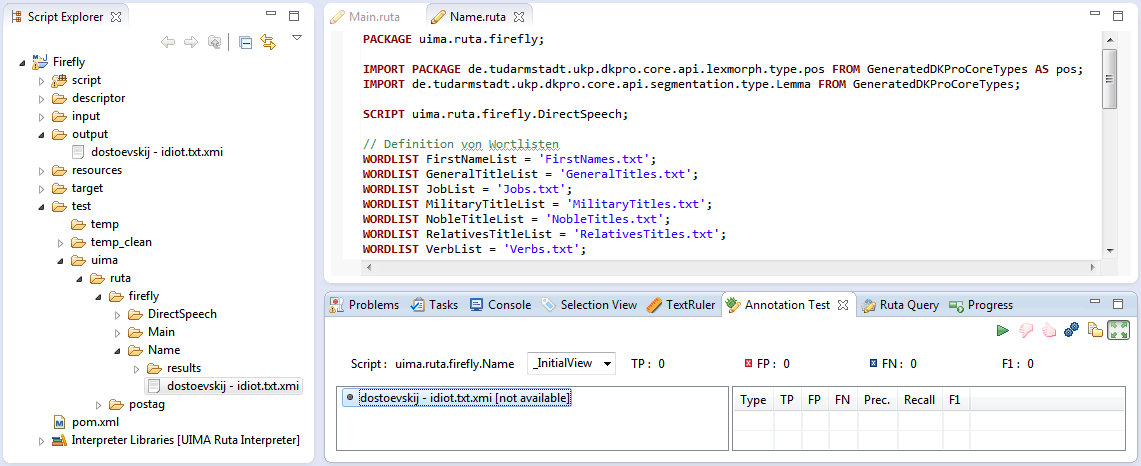
\includegraphics[width=1\textwidth]{figs/test_main.png}
\caption{Im \textit{Script Explorer} ist die Struktur des Testordner zu erkennen. Das relevante Skript muss angeklickt werden, damit unten der \textit{Annotation Test} angezeigt wird.}
\label{test_main}
\end{figure}

Auf der linken Seite ist der \textit{Script Explorer} mit allen Unterordnern von \textit{test}. Das zu testende Dokument wird in den entsprechenden Ordner eingefügt. Testen wir also das Skript \textit{Name.ruta}, kopieren wir das Referenzdokument in den Unterordner \textit{Name}. Der Unterordner \textit{results} enthält die Ergebnisdateien des \textit{Annotation Test}. Neben den ursprünglichen Annotationstypen sind zusätzlich die Typen \textit{TruePositive}, \textit{FalsePositive} und \textit{FalseNegative} gespeichert. \textit{TruePositive} sind dabei die richtig markierten Abschnitte. Alle \textit{FalsePositive} sind fälschlicherweise markiert, während hingegen alle \textit{FalseNegative} fälschlicherweise nicht markiert sind. Die Anzahl dieser Typen ist im \textit{Annotation Test} bei \textit{TP}, \textit{FP} und \textit{FN} zu finden. Der \textit{F1-Wert} liegt im Zahlenbereich zwischen 0 und 1. Umso höher der Wert, desto besser die Trefferquote. Wenn ein Test gestartet werden soll, wird der grüne Pfeil gedrückt. Da das derzeitige Referenzdokument eine exakte Kopie des Ausgabedokumentes ist, gibt es nur \textit{TruePositives} und der F1-Wert ist genau 1. Wird einer der beiden Daumen gedrückt, erscheint das Auswahlfenster (Abb.~\ref{thumb}), in dem sämtliche Annotationstypen ausgewählt werden können. Der \glqq Daumen nach unten\grqq{} lässt uns Annotationstypen auswählen, die wir nicht testen wollen, wohingegen der \glqq Daumen nach oben\grqq{} zwischen den relevanten Typen auswählen lässt.

\begin{figure}
\centering
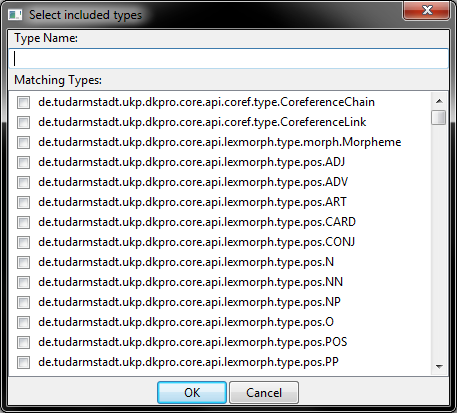
\includegraphics[width=0.5\textwidth]{figs/test_thumb.png}
\caption{Auswahl relevanter oder irrelevanter Annotationstypen.}
\label{thumb}
\end{figure}

Daneben können bei den beiden Zahnrädern weitere Ein\-stel\-lungs\-mög\-lich\-kei\-ten vorgenommen werden (Abb.~\ref{test_pref}). Das Aktivieren von \textit{Use all types} stellt sicher, dass zunächst alle Typen zum Test genutzt werden, außer man spezialisiert seine Suche mit Hilfe der Typenwahl (Abb.~\ref{thumb}). Der Punkt \textit{Extend classpath} sollte aktiviert sein, wenn wir TreeTagger nutzen, da sonst kein Test durchgeführt werden kann. Unter \textit{Evaluator} kann die Art der Übereinstimmung gewählt werden. Bei \textit{Exact Match} muss das Ergebnis exakt der Referenzannotation entsprechen, während \textit{Partial Match} auch bei teilweise richtiger Markierung ein \textit{TruePositive} liefert.

\begin{figure}
\centering
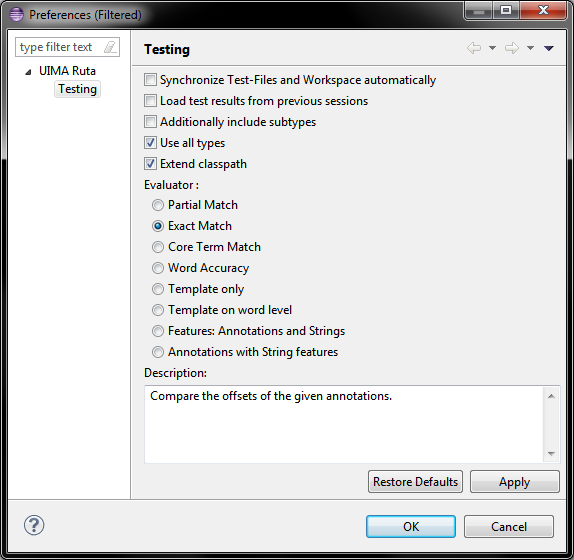
\includegraphics[width=0.5\textwidth]{figs/test_pref.png}
\caption{Einstellungen des \textit{Annotation Test}.}
\label{test_pref}
\end{figure}

Das vorletzte Symbol aus Abb.~\ref{test_main} exportiert das Testergebnis als Tabelle in einer CSV-Datei, während das Letzte die Option \textit{Extend classpath} symbolisiert. Im Moment haben wir noch kein nutzbares Referenzdokument, da wir lediglich das Ausgabedokument in den Testordner kopiert haben. Deswegen müssen wir das Dokument im Testordner mit allen richtigen Annotationen versehen. Dazu öffnen wir das Dokument mit einem Doppelklick und wählen im \textit{Annotation Browser View} alle Annotationstypen aus, die wir bearbeiten wollen. In unserem Beispiel ist das \textit{FirstName}, \textit{LastName} und \textit{PersName}, weil wir später nur die Trefferquote dieser Typen überprüfen wollen. Finden wir eine Person, müssen wir zunächst bestimmen, zu welchem Annotationstyp diese gehört. In Abb.~\ref{annotate} ist \glqq Rogoschin\grqq{} weder als \textit{LastName}, noch als \textit{PersName} markiert. Wir annotieren das Wort mit \textbf{Doppelklick $\rightarrow$ Rechtsklick $\rightarrow$ Annotate $\rightarrow$ LastName} als \textit{LastName}.

\begin{figure}
\centering
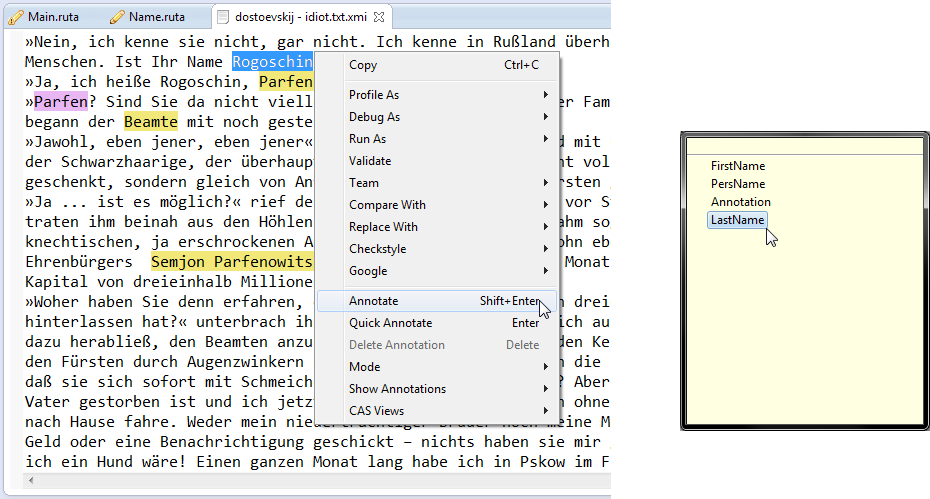
\includegraphics[width=0.75\textwidth]{figs/test_annotate.png}
\caption{Manuelles Annotieren der Referenzdatei mit \textit{Annotate}.}
\label{annotate}
\end{figure}

Es werden nur diejenigen Wörter als \textit{PersName} markiert, die keine Namen sind, z.B. \glqq Schwarzhaarige\grqq{}. Dies spart uns in diesem Text viel Zeit, da wir im Anschluss mit \textit{Quick Annotate} schneller arbeiten. Sind also alle Namen als \textit{FirstName} bzw. \textit{LastName} und jedes Synonym als \textit{PersName} markiert, verändern wir den Annotationsmodus. Dazu klicken wir im Text auf \textbf{Rechtsklick $\rightarrow$ Mode} und navigieren zu \textit{PersName}, wie in Abb.~\ref{mode}. Jetzt kann das gesamte Dokument überflogen werden, ohne jeden Satz lesen zu müssen. Jede vorhandene Annotation wird markiert und mit \textbf{Enter} als \textit{PersName} markiert. Natürlich sollen die zuvor markierten \textit{PersName} nicht wiederholt markiert werden. Außerdem ist darauf zu achten, dass beispielsweise \glqq Parfen Rogoschin\grqq{} als Ganzes markiert wird, nicht einzeln. Auch ist beispielsweise \glqq Generalin Jepantschina\grqq{} ein \textit{PersName}, da der General und die Generalin zwei unterschiedliche Personen sind.

\begin{figure}
\centering
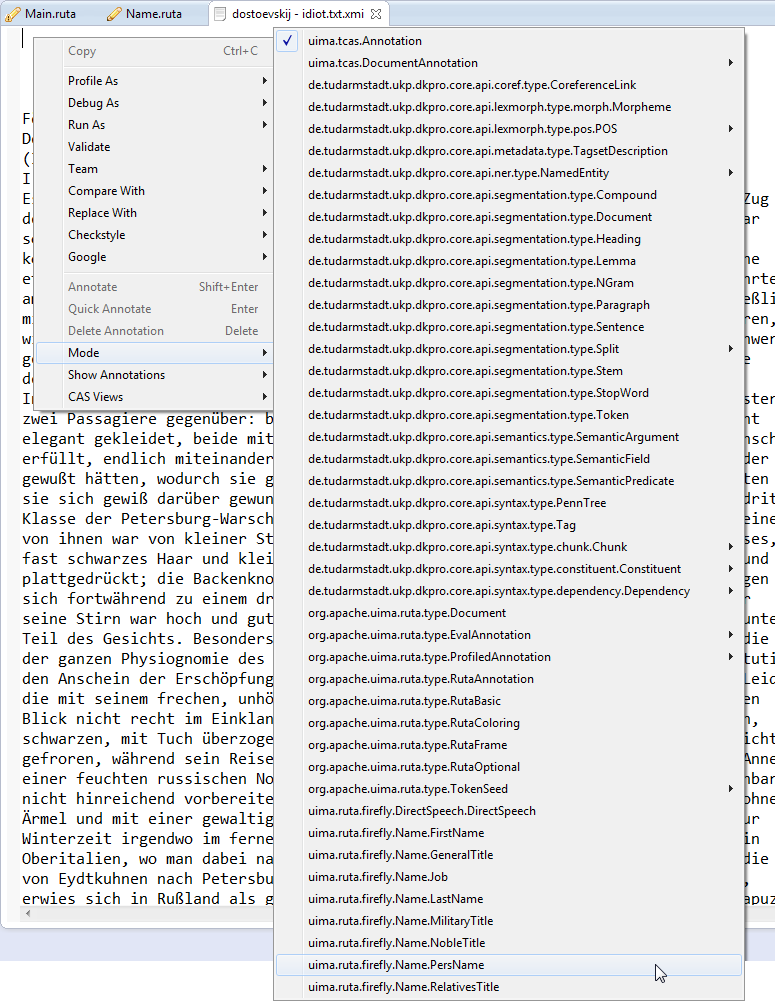
\includegraphics[width=0.5\textwidth]{figs/test_mode.png}
\caption{Ändern des Annotationsmodus über \textit{Mode}.}
\label{mode}
\end{figure}

\newpage

Zusätzlich gibt es die Möglichkeit, eine Annotation zu entfernen. Dies ist notwendig, da wir das Referenzdokument aus dem \textit{output} Ordner kopiert haben und dort möglicherweise falsche Annotationen vorhanden sind. Die erste Option ist es, in den jeweiligen Annotationsmodus zu wechseln und die Annotation mit \textbf{Entf} bzw. \textbf{Del} zu entfernen. Bei der zweiten Option müssen wir die jeweilige Annotation im \textit{Annotation Browser View} suchen und ebenfalls mit \textbf{Entf} löschen.

\subsection{Fehleranalyse und Verbesserung}

Ist das gesamte Dokument vollständig mit Annotationstypen versehen, kann der \textit{Annotation Test} gestartet werden. Dazu wählen wir nur die Typen \textit{FirstName}, \textit{LastName} und \textit{PersName} aus und starten den Test. Das Ergebnis ist in Abb.~\ref{test_result} zu sehen.

\begin{figure}
\centering
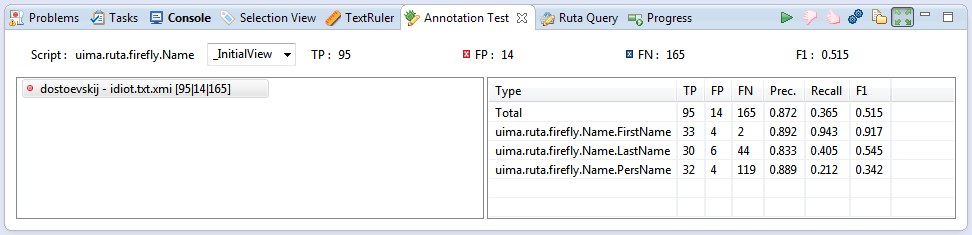
\includegraphics[width=1\textwidth]{figs/test_result.png}
\caption{Der erste Test mit dem unangepassten Skript findet gerade 32 Personen.}
\label{test_result}
\end{figure}

Der F1-Wert liegt bei über 0.5. Wenn wir jedoch den Wert in der Zeile von \textit{PersName} betrachten, sehen wir, dass wir nur knapp 20\,\% der Personen gefunden haben. Wenn wir wissen wollen, woran das liegt und wie das verbessert werden kann, öffnen wir das Ergebnisdokument mit einem Doppelklick im Fenster links. Im \textit{Annotation Browser View} markieren wir die Typen \textit{TruePositive}, \textit{FalsePositive} und \textit{FalseNegative}, um uns einen ersten Überblick des Ergebnisses zu verschaffen. Außerdem ordnen wir die Ansicht der Fenster per Drag\&Drop um, sodass wir schnell eine Liste der Treffer haben (Abb.~\ref{test_view}).

\begin{figure}
\centering
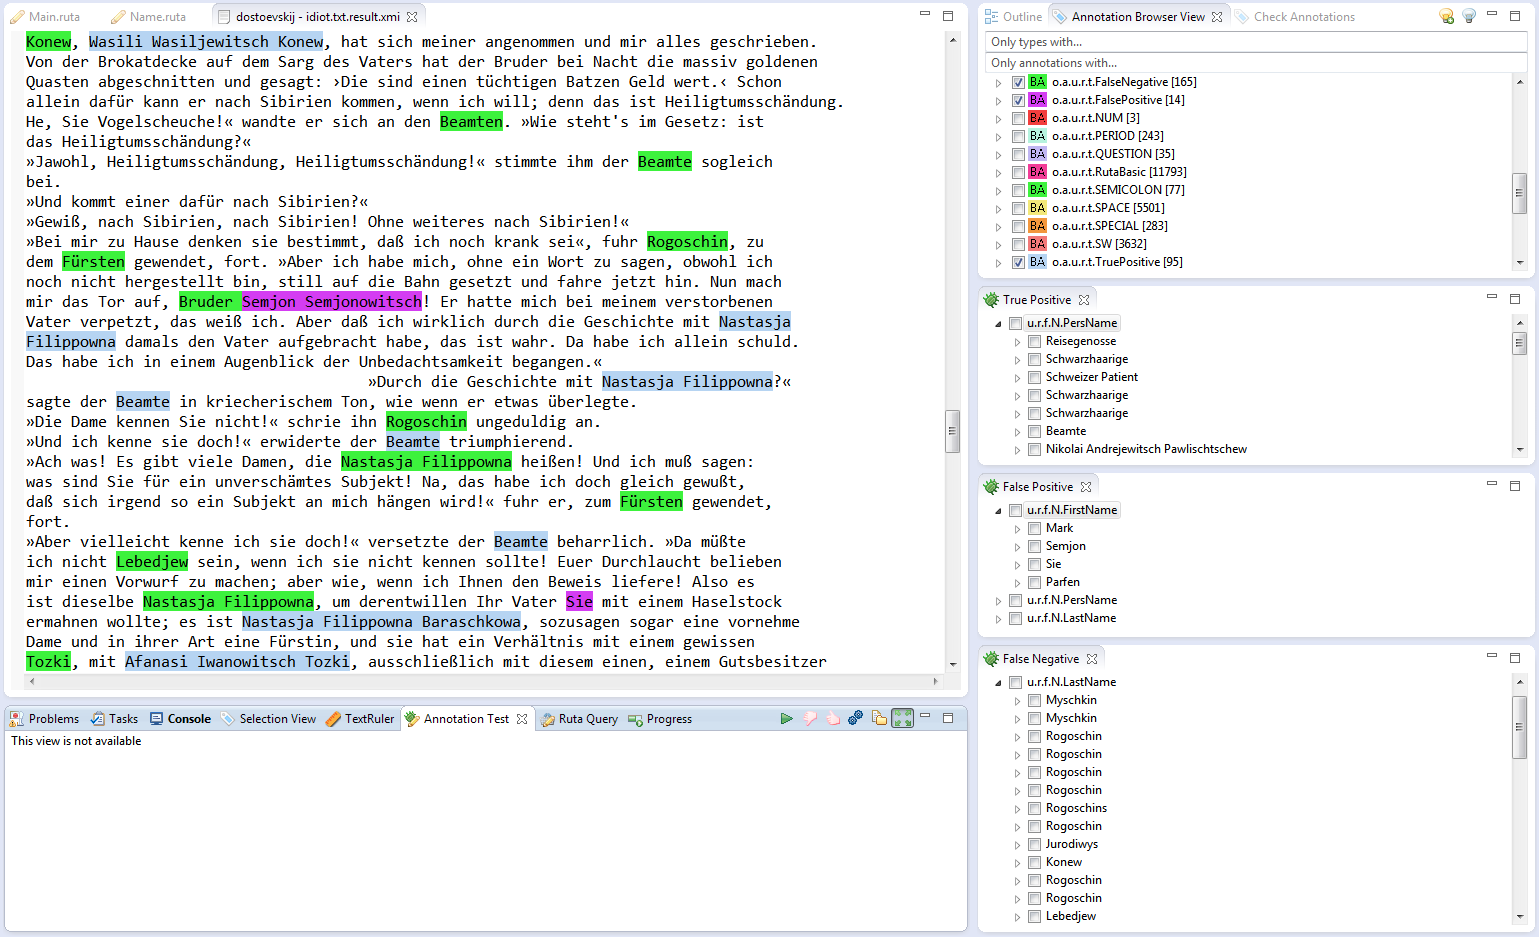
\includegraphics[width=1\textwidth]{figs/test_view.png}
\caption{Im linken Fenster sind alle \textit{TruePositive}, \textit{FalsePositive} und \textit{FalseNegative} markiert. In der rechten Ansicht ist eine detaillierte Übersicht der (nicht) gefundenen Vornamen, Nachnamen und Personen.}
\label{test_view}
\end{figure}

Wir sehen, dass viele Namen zuverlässig gefunden wurden, aber die gleiche Person an einer anderen Textstelle nicht. Das liegt daran, dass wir beispielsweise \glqq Herr Rogoschin\grqq{} finden, nicht aber ein einzeln stehendes \glqq Rogoschin\grqq{}. Des Weiteren gibt es auch noch keine Regel die eine Abwandlung der Namen, wie \glqq Rogoschins\grqq{}, findet. Um das zu beheben gibt es nicht nur statische Wortlisten, sondern auch dynamische Stringlisten. Diese werden mit dem Befehl \texttt{STRINGLIST} erstellt und beinhalten \texttt{STRING} Elemente, die wir in die Regeln einbauen werden. Das vollständige Skript ist im Quelltext~\ref{final_rules} zu sehen.

\begin{Ruta}[caption={Das finale Skript Name.ruta.}\label{final_rules}]
PACKAGE uima.ruta.firefly;

IMPORT PACKAGE de.tudarmstadt.ukp.dkpro.core.api.lexmorph.type.pos
FROM GeneratedDKProCoreTypes AS pos;
IMPORT de.tudarmstadt.ukp.dkpro.core.api.segmentation.type.Lemma
FROM GeneratedDKProCoreTypes;

SCRIPT uima.ruta.firefly.DirectSpeech;

// Definition von Wortlisten
WORDLIST FirstNameList = 'FirstNames.txt';
WORDLIST GeneralTitleList = 'GeneralTitles.txt';
WORDLIST JobList = 'Jobs.txt';
WORDLIST MilitaryTitleList = 'MilitaryTitles.txt';
WORDLIST NobleTitleList = 'NobleTitles.txt';
WORDLIST RelativesTitleList = 'RelativesTitles.txt';
WORDLIST VerbList = 'Verbs.txt';

// Definition von Stringlisten und Stringvariable
STRINGLIST FirstNames;
STRINGLIST LastNames;
STRINGLIST PersNames;
STRING MatchedName;

// Deklaration neuer Annotationstypen
DECLARE FirstName, LastName, PersName,
GeneralTitle, Job, MilitaryTitle, NobleTitle, RelativesTitle;

// Importierte Skripte ausfuehren
Document{-> CALL(DirectSpeech)};

// Abgleichen der Wortlisten mit input
Document{-> MARKFAST(FirstName, FirstNameList)};
Document{-> MARKFAST(GeneralTitle, GeneralTitleList)};
Document{-> MARKFAST(Job, JobList)};
Document{-> MARKFAST(MilitaryTitle, MilitaryTitleList)};
Document{-> MARKFAST(NobleTitle, NobleTitleList)};
Document{-> MARKFAST(RelativesTitle, RelativesTitleList)};

// VORNAMEN
// Folgt nach einem RelativesTitle ein grossgeschriebenes Wort,
// so wird CW als FirstName markiert und in die Liste FirstNames gespeichert
RelativesTitle pos.N{-PARTOF(FirstName) ->
MARK(FirstName), MATCHEDTEXT(MatchedName), ADD(FirstNames, MatchedName)};
// An alle Vornamen ein "s" haengen und in FirstNames speichern
FirstName{-> MATCHEDTEXT(MatchedName), ADD(FirstNames, MatchedName + "s")};
// Vornamen aus der Liste FirstNames markieren
CW{-PARTOF(FirstName), INLIST(FirstNames) -> MARK(FirstName)};
// Vorname + Vorname = Vorname
FirstName{-> SHIFT(FirstName, 1, 2)} FirstName{-> UNMARK(FirstName)};

// NACHNAMEN
// Folgt nach einem Firstname ein grossgeschriebenes Wort,
// so wird CW als LastName markiert und in die Liste LastNames gespeichert
FirstName pos.N{->
MARK(LastName), MATCHEDTEXT(MatchedName), ADD(LastNames, MatchedName)};
// Folgt nach einem der Titel ein grossgeschriebenes Wort,
// so wird CW als LastName markiert
(GeneralTitle|Job|MilitaryTitle|NobleTitle) pos.N{-PARTOF(LastName)
-> MARK(LastName), MATCHEDTEXT(MatchedName), ADD(LastNames, MatchedName)};
// An alle Nachnamen ein "s" haengen und in LastNames speichern
LastName{-> MATCHEDTEXT(MatchedName), ADD(LastNames, MatchedName + "s")};
// Nachnamen aus der Liste LastNames markieren
CW{-PARTOF(LastName), INLIST(LastNames) -> MARK(LastName)};

// PERSONEN
// Das Vorkommen eines ganzen Namens (Vorname + Nachname),
// als PersName markieren
(RelativesTitle|GeneralTitle|Job|MilitaryTitle|NobleTitle)* @FirstName
LastName{-> MARK(PersName, 1, 2, 3)};
(RelativesTitle|GeneralTitle|Job|MilitaryTitle|NobleTitle)* @FirstName
{-PARTOF(PersName) -> MARK(PersName, 1, 2)};
(RelativesTitle|GeneralTitle|Job|MilitaryTitle|NobleTitle)* @LastName
{-PARTOF(PersName) -> MARK(PersName, 1, 2)};
// Sprecher nach einer direkten Rede erkennen
DirectSpeech COMMA? pos.V{INLIST(VerbList, Lemma.value)} pos.ART CW+
{-> MARK(PersName), MATCHEDTEXT(MatchedName), ADD(PersNames, MatchedName)};
// Personen aus der Liste PersNames markieren
CW{-PARTOF(PersName), INLIST(PersNames) -> MARK(PersName)};
\end{Ruta}

\newpage

Für jeden Abschnitt haben wir eine Stringliste definiert, da wir diese am Ende jedes Abschnitts verwenden. In die Stringvariable schreiben wir einen gefundenen Namen bzw. Person, um ihn in eine Liste speichern zu können. Die erste Regel wurde so erweitert, dass mit \texttt{MATCHEDTEXT} der potenzielle Vorname in den String \textit{MatchedName} gespeichert wird. Anschließend fügen wir mit \texttt{ADD} den gefundenen Vornamen in unsere Stringliste, in die alle Vornamen gespeichert werden, die nicht in der Wortliste \textit{FirstNameList} sind. Zusätzlich wurde \texttt{CW} durch \texttt{pos.N} ersetzt, da wir sonst auch Wörter wie \glqq Sie\grqq{} finden würden, das zu den Pronomen gehört und nicht zu den Nomen. Im zweiten Schritt suchen wir nochmals nach Vornamen, schreiben diese aber mit einem angehängten \glqq s\grqq{} in die Stringliste, um so auch kleine Abwandlungen von Namen zu finden. Die nächste neue Regel untersucht alle \texttt{CW} im Text und prüft mit \texttt{INLIST}, ob es in unserer Liste \textit{FirstNames} gibt. Bei jeder Regel ist zu beachten, dass wir einen schon markierten Abschnitt nicht doppelt annotieren. Im Skript \textit{Name.ruta} verhindern wir mögliche Probleme, da \texttt{-PARTOF} dies ausschließt. Der zweite Abschnitt ist nach dem selben Prinzip erweitert worden, wie der Erste. Potenzielle Nachnamen werden in eine Liste geschrieben, Abwandlungen werden gespeichert und zum Schluss annotiert. Der letzte Abschnitt fügt Titel, Vornamen und Nachnamen zu einer Person zusammen. Jeder Annotationstyp, der mit einem Stern (\texttt{*}) endet, kann keinmal oder mehrmals vorkommen. Das Zeichen \texttt{@} vor einem Annotationstyp heißt, dass UIMA Ruta zuerst nach diesem im Text sucht und dann prüft, ob die restliche Regel zutrifft. Bei richtiger Nutzung führt dies zu einer Geschwindigkeitssteigerung. Personen nach direkten Reden werden ebenfalls in einer Liste gespeichert und anschließend im gesamten Text gefunden. Wenn das Skript erneut getestet wird, können wir eine erhebliche Steigerung des Ergebnisses erkennen (Abb.\ref{final_result}). 

\begin{figure}
\centering
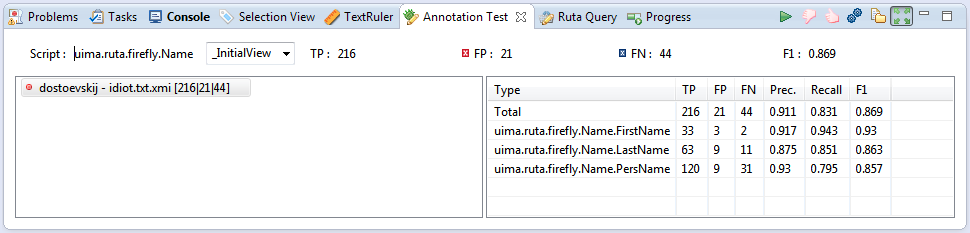
\includegraphics[width=1\textwidth]{figs/final_result.png}
\caption{Das Endergebnis des Beispiels zeigt eine Steigerung der (korrekt) gefundenen Personen von 32 auf 120.}
\label{final_result}
\end{figure}

Mit den vorgestellten Techniken von UIMA Ruta, der Textanalyse, TreeTagger und dem \textit{Annotation Test} kann sehr schnell eine hohe Trefferquote erzielt werden. Mit Hilfe des \textit{Annotation Test} muss zum Schluss jede Regel weiter verfeinert werden, bis ein akzeptables Niveau erreicht ist.

\end{document}